\documentclass[diss]{template/setrem}
\sloppy
\usepackage[utf8]{inputenc}
\usepackage[table]{xcolor}
\usepackage{multicol}
\usepackage{array} % for defining a new column type
\usepackage{varwidth} %for the varwidth minipage environment
\usepackage{float}
\usepackage{todonotes}
\usepackage{subfigure}
\usepackage{graphicx,url}
\usepackage{lipsum} %generate fake text

\makeatletter
\g@addto@macro{\UrlBreaks}{\UrlOrds}
\makeatother


\usepackage{setspace}
\usepackage{amssymb}
\usepackage{colortbl}
\usepackage{color}
\usepackage{hyperref}
\usepackage{verbatim}
\usepackage{scrextend}
\usepackage{csvsimple}
\usepackage{glossaries}

\usepackage{listings}
\usepackage{xcolor}
\usepackage{threeparttablex}
\usepackage{lscape}
\usepackage{colortbl}
\usepackage{booktabs}

% Coloca a contagem das figuras sequenciais sem considerar capítulos
\usepackage{chngcntr}
\usepackage{tabularx}
\usepackage{amsmath}
\usepackage{datatool}
\usepackage{seqsplit}
% \usepackage[toc,page]{appendix}
\usepackage[titletoc, title]{appendix}
\usepackage{longtable}
\usepackage{multirow}
\usepackage{titletoc}
\usepackage{pdfpages}

\makeatletter
\def\@cline#1-#2\@nil{%
  \omit
  \@multicnt#1%
  \advance\@multispan\m@ne
  \ifnum\@multicnt=\@ne\@firstofone{&\omit}\fi
  \@multicnt#2%
  \advance\@multicnt-#1%
  \advance\@multispan\@ne
  \leaders\hrule\@height\arrayrulewidth\hfill
  \cr
  \noalign{\nobreak\vskip-\arrayrulewidth}}
\makeatother


\counterwithout{figure}{chapter}
\counterwithout{table}{chapter}

\definecolor{color_keywords}{rgb}{0.0, 0.0, 0.44}
\definecolor{color_mykeyword}{RGB}{10, 100, 112}

\definecolor{myblue}{rgb}{0,0.3,0.9}
\definecolor{mygreen}{rgb}{0,0.6,0}
\definecolor{mygray}{rgb}{0.5,0.5,0.5}
\definecolor{mymauve}{rgb}{0.58,0,0.82}
\definecolor{mygray2}{rgb}{0.2,0.2,0.2}
\definecolor{mygray3}{rgb}{0.4,0.4,0.4}



\lstdefinestyle{mycode}{ %
  %backgroundcolor=\color{yellow!05},   % choose the background color; you must add \usepackage{color} or \usepackage{xcolor}
  basicstyle=\linespread{1}\small,        % the size of the fonts that are used for the code \footnotesize
  %lineskip={-1pt},
  breakatwhitespace=false,         % sets if automatic breaks should only happen at whitespace
  breaklines=true,                 % sets automatic line breaking
  captionpos=t,                    % sets the caption-position to top
  commentstyle=\color{gray!90},    % comment style
%  deletekeywords={...},            % if you want to delete keywords from the given language
  escapeinside={\%*}{*)},          % if you want to add LaTeX within your code
  extendedchars=true,              % lets you use non-ASCII characters; for 8-bits encodings only, does not work with UTF-8
  frame=l,                    % adds a frame around the code (bt,l,r) single
  keepspaces=true,                 % keeps spaces in text, useful for keeping indentation of code (possibly needs columns=flexible)
  keywordstyle=\color{black}\bf,       % keyword style
  language=C++,                     % the language of the code
 % morekeywords={input,output,parallel_activity,stream_producer},            % if you want to add more keywords to the set
  keywordstyle=[2]{\color{blue}\bf},
 % keywords=[3]{serial_in_order, parallel, pipeline, run, add_filter, task_scheduler_init},
 % keywordstyle=[3]{\color{blue!70!green}\bf},
  numbers=left,                    % where to put the line-numbers; possible values are (none, left, right)
  numbersep=5pt,                   % how far the line-numbers are from the code
  numberstyle=\tiny\color{mygray}, % the style that is used for the line-numbers
  rulecolor=\color{black},         % if not set, the frame-color may be changed on line-breaks within not-black text (e.g. comments (green here))
  showspaces=false,                % show spaces everywhere adding particular underscores; it overrides 'showstringspaces'
  showstringspaces=false,          % underline spaces within strings only
  showtabs=false,                  % show tabs within strings adding particular underscores
  stepnumber=1,                    % the step between two line-numbers. If it's 1, each line will be numbered
  stringstyle=\color{red},     % string literal style
  tabsize=1,                       % sets default tabsize to 2 spaces
  title=\lstname                   % show the filename of files included with \lstinputlisting; also try caption instead of title
}

% Negrito no título do listing
\captionsetup[lstlisting]{font={bf},labelfont=bf}

%Ajusta a contagem do listing
\AtBeginDocument{% the counter is defined later
  \counterwithout{lstlisting}{chapter}%
}
\makeatletter
\renewcommand{\l@lstlisting}[2]{%
  \@dottedtocline{1}{0em}{1.5em}{\lstlistingname\ #1}{#2}%
}
\makeatother


\title{Desenvolvimento de um app mobile para chamados de suporte de uma empresa}
\author{Giehl}{Bruno Leonardo}
\author{Conrad}{Mateus Augusto}
\advisor{Msc.}{Siqueira}{Denise}
\advisor{Esp.}{Knob}{Alexandre}
%%%%%ARRUMAR ISSO


% Place where the undergraduate thesis will be made.
\location{Três de Maio}{RS}

% Date of undergraduate thesis development/presentation.
\date{Setembro}{2019}

% Course name - defined in setremdefs.sty.
\course{\ctrc}
%\vspace{-4cm}

% Header image of the cover.

% Sistemas de Informação
\courseheader{\silogo[1]}

\docname{Relatório Final do Trabalho Interdisciplinar III do Curso de Bacharelado em Sistemas de Informação - Faculdade Três de Maio - SETREM}

% Mostra a lista de tabelas e figuras com os prefixos corretos.
\titlecontents{table}
  [0em]
  {}
  {\tablename\enspace\thecontentslabel:\enspace\enspace}
  {}
  {\titlerule*[.5pc]{.}\contentspage}

\titlecontents{figure}
  [0em]
  {}
  {\figurename\enspace\thecontentslabel:\enspace\enspace}
  {}
  {\titlerule*[.5pc]{.}\contentspage}

\begin{document} 
\maketitle
%\input{apro.tex}
\begin{abstract}

Today, companies in all industries use some form of IT infrastructure and services to run their business. This is mainly due to the ability to improve the business through the implementation of ERP'S and other tools, capable of controlling the business flow, as well as presenting concrete and real time data about the business. The IT infrastructure needs constant support so that downtime in the event of equipment failures / errors required for the full operation of the operation to have the least possible impact, and for this reason, medium to large companies employ their own management team. support, usually operating as a service desk. Thus, the present work proposes the development of a mobile application for Android operating systems, to open and support IT support calls, aiming to facilitate and standardize the service process using the ITIL guide for good practice in IT. IT as well as graphing for easy viewing of recurring information. This research and development took place with the object of research the environment of the IT support sector of the company Abase Sistemas Ltda. Application development is treated as the main problem of the present research, in which the existing methodologies in the company were analyzed, so that the real needs and functionalities necessary to propose a solution capable of standardizing the support were analyzed. The application has access levels for attendants and users, allowing you to create tickets, and track the status of the ticket, having its development based on the Dart language plus the Flutter framework, as well as using Firebase non-relational database. Through this research, it was possible to develop an application following the requirements raised through the evaluation of the company's IT sector, as well as presenting useful information to users through the generation of graphs. 
\end{abstract}
\keyw{Support. Development. Information technology}

\begin{resumo}

.Nos dias atuais, empresas de todos setores do mercado se utilizam de alguma forma de infraestruturas e/ou serviços de TI para conduzir seu negócio. Isso se deve principalmente pela capacidade de aprimoramento do negócio através da implementação de ERP’S e demais ferramentas, capazes de controlar o fluxo de negócio, além de apresentar dados concretos e em tempo real acerca do negócio. A infraestrutura de TI necessita de constante suporte para que o \textit{downtime} em casos de falhas/erros nos equipamentos necessários para o pleno funcionamento da operação cause o mínimo impacto possível, e, por esta razão, empresas de médio a grande porte empregam sua própria equipe de suporte, costumeiramente operando como uma central de serviços. Sendo assim, o presente trabalho propõe o desenvolvimento de uma aplicação mobile para sistemas operacionais Android, para realizar abertura e atendimento de chamados de suporte de TI, visando facilitar e padronizar o processo de atendimento utilizando-se ainda do guia de ITIL para boas prática em TI, bem como a geração de gráficos para facilitar a visualização de informações recorrentes. A presente pesquisa e desenvolvimento ocorreram tendo como objeto de pesquisa  o ambiente do setor de suporte de TI da empresa Abase Sistemas Ltda. O desenvolvimento da aplicação é tratada como a principal problemática da presente pesquisa, na qual foram analisadas as metodologias já existentes na empresa, para que assim se avaliasse as reais necessidades e funcionalidades necessárias para propor uma solução capaz de padronizar o suporte. A aplicação apresenta níveis de acesso para atendentes e usuários, permitindo criar chamados, e acompanhar o status do chamado, tendo seu desenvolvimento baseado na linguagem Dart acrescida do framework Flutter, bem como utilização de banco de dados não-relacional Firebase. Através da presente pesquisa, foi possível desenvolver uma aplicação seguindo os requisitos levantados através da avaliação do setor de TI da empresa, bem como apresentar informações úteis aos usuários através da geração de gráficos.
\end{resumo}
\keyw{Suporte. Desenvolvimento. Tecnologia da Informação.}

\begin{singlespaced}    %Lista de figuras
    \listoffigures
\end{singlespaced}

\begin{singlespaced}    %Lista de tabelas
    \listoftables
\end{singlespaced}

\begin{listofabbrv}{OR-AC-GAN} % Lista de siglas.
    \setstretch{1}
    \item[ACM] {Association for Computing Machinery}
    \item[API] {Applicatio Programming Inteafce}
    \item[BaaS] {Back-end as a Service}
    \item[COBIT]{Control Objectives for Information and related Technology}
    \item[COSO] {Committee of Sponsoring Organizations}
    \item[GCP] {Google Cloud Platform}
    \item[GITIM]{Government Information Technology Infraestructure Method}
    \item[IBGE] {Instituto Brasileiro de Geografia e Estatísticas}
    \item[ITIL] {Information Technology Infrastructure Library}
    \item[JSON] {JavaScript Object Notation}
    \item[MVC] {Model View and Controller}
    \item[NoSQL]{Not Only SQL}
    \item[TI]{Tecnologia da informação}
    \item[RDM]{Requisições de Mudança}
    \item[RF]{Requisito Funcional}
    \item[RNF]{Requisito Não Funcional}
    \item[SDK]{Software Development Kit}
    \item[SGBD]{Sistema Gerenciador de Banco de Dados}
    \item[SGBDTR]{Sistema Gerenciador de Banco de Dados em Tempo Real}
    \item[SQL]{Structured Query Language} 
\end{listofabbrv}
\tableofcontents
\chapter*{Introdução} \label{chap:intro}

A tecnologia da informação pode ser considerada como um conjunto de tecnologias para processar e armazenar dados com o uso de hardware, software, comunicação e pessoas. A TI, na verdade, procura facilitar processos através da eliminação de rotinas que possam ser muito repetitivas e também reduzir a quantidade de erros operacionais de usuários. 

Assim como qualquer área de negócio, a TI tem a necessidade de ser gerenciada, então surge a área de gerenciamento de serviços de TI. Essa gestão procura usar soluções de software ou até mesmo mudanças de metodologias internas para atingir mais agilidade nos processos. Também pode ser colocada como a prática estruturada de se indicar as formas mais adequadas de atender as necessidades tecnológicas uma organização. 

Para realizar isso o gerenciamento de serviços de TI deve ter a avaliação dos recursos tecnológicos disponíveis, determinar quais as restrições de recursos, implementar as mudanças e otimizações no serviço de TI para procurar remover as restrições, gerenciar as melhorias de forma integrada, fazer o monitoramento dos resultados, procurar avaliar a necessidade de novas otimizações e atualizações dos serviços de TI, atender chamados, quando necessário, e, por fim, procurar diminuir ocorrências, principalmente as ocorrências com repetição frequente.

Os dispositivos móveis traçaram um longo caminho nos últimos anos. Por um tempo, os  celulares eram apenas usados com o intuito fazer ligações. Todavia, a medida que esses dispositivos continuavam evoluindo, a capacidade de enviar e receber mensagens de texto e multimídia, criar agendas e salvar contatos tornou-se prontamente disponível. Atualmente os dispositivos móveis são usados em larga escala e são capazes de atender a diversos outros propósitos.

O uso de um software, como um app mobile devido a popularidade dos smartphones, direcionado a gestão de ti permitira ter sempre em mãos a capacidade de controlar os serviços de TI da empresa. Portanto, surge a necessidade de desenvolver um app para criar, monitorar e gerenciar chamados de suporte interno de uma organização. Tendo isso em vista, é necessário procurar embasamento referente a metodologias e boas praticas de gerenciamento de ti.

Um dos primeiros conceitos a se observar ao se discutir sobre gerenciamento de TI é ITIL. O ITIL é uma biblioteca que reúne um conjunto de boas praticas para gerenciamento de TI, que nesse escopo trata sobre a central de serviços, gerenciamento de incidentes, de problemas, de configurações e de mudanças.

No que diz respeito a desenvolvimento de apps mobile, é possível encontrar diversas linguagens de programação e frameworks pra auxiliar no processo, então deve-se optar pela alternativa que leva mais em conta em termos de produtividade, qualidade e inovação. 

O uso do Flutter pode se adequar em relação a produtividade, pois com apenas um código é capaz de gerar aplicativos com performance nativa para smartphones Android e Ios. Qualidade de desenvolvimento pode ser algo relativo, sendo necessária uma análise de experiência de usuário para ser possível dizer o que tem mais qualidade.

Além do desenvolvimento da interface e funcionamento do app, é necessário um meio de controlar os dados gerados através do app. Em consequência disso, pode-se buscar inovar no que diz respeito a infraestrutura do próprio aplicativo, ou seja, usar de softwares como serviço para o back-end em \textit{cloud} para fazer \textit{storage} de arquivos, estruturação de dados e funções personalizadas para o próprio aplicativo.
\chapter{Projeto de Pesquisa} \label{chap:ResearchPlan}

\section{Tema} \label{sec::Theme}
Análise e desenvolvimento de um aplicativo mobile para realizar e atender chamados de suporte interno.

\subsection{Delimitação do Tema} \label{subsec::ThemeDelimitation}
A delimitação do projeto se dará a análise e desenvolvimento de uma aplicação mobile de chamados de suporte interno - help desk -  em uma empresa de software aplicando o guia de boas práticas da ITIL. A pesquisa será desenvolvida pelos acadêmicos Bruno Leonardo Giehl e Mateus Augusto Conrad no período compreendido entre Agosto e Dezembro de 2019, em parceria com a empresa Abase Sistemas e Soluções Ltda, na qual a pesquisa será desenvolvida.

%objetivos
\section{Objetivos} \label{sec:objective}
O objetivo visa identificar, de forma abrangente, a proposta para solução do problema proposto e o mesmo deve ser descrito com verbos no infinitivo \citep{lovato_2007}.

\subsection{Objetivo Geral}
O objetivo geral do trabalho é desenvolver um aplicativo para padronizar o processo de abertura de chamados de suporte internos de uma empresa de TI.
%objetivos específicos
\subsection{Objetivos Específicos}
\begin{enumerate}
    \item Fazer a análise e desenvolvimento de um app para chamados de suporte.
    \item Usar um banco de dados em tempo real para gerenciamento dos dados
    \item Fazer os testes de Software no aplicativo 
    \item Disponibilizar o arquivo para instalação do app.
\end{enumerate}

\section{Justificativa}\label{sec:justification}
De acordo com \citet{marconi_lakatos_2010}, a justificativa possui o objetivo de apresentar o porquê de algo estar sendo realizado. A mesma faz uso de recursos teóricos e práticos para assim conseguir alcançar seu objetivo. A Justificativa serve, principalmente para justificar a pesquisa e convencer o leitor ou orientador da mesma.

O trabalho pode ser justificado a partir de dois principais fatores: o porquê desenvolver mobile, o porquê usar de conceitos de gerenciamento de TI e também o motivo de unir esses dois fatores. 

O avanço da tecnologia aplicada em smartphones e a maneira de como as empresas modernas estão se comportando está mudando constantemente. A partir do momento que se há um negócio em desenvolvimento ou se está começando a desenvolver algo, ter acesso o acesso do mesmo por um aplicativo para smartphone é fundamentalmente considerável, isso devido a quantidade de usuários nessa plataforma. De acordo com uma pesquisa realizada pelo IBGE, o acesso a internet já era 69\% proveniente de smartphones em 2016, ou seja, além do crescente número de acessos por smartphones, diminui o número de acessos por computadores.

No quesito de desenvolvimento mobile, há discussões envolvendo o uso de desenvolvimento de páginas web responsivas ao invés de aplicativos instalados no dispositivo do usuário. Apesar de muitas vezes aplicativos sites responsivos oferecerem a mesma funcionalidade, ter um aplicativo pode diminuir o tempo de espera de carregamento de páginas, justamente pelo fato de não necessitar de         tantas requisições para o servidor da aplicação. Outro fator contra o uso de páginas web é o uso de uma conexão de qualidade ruim, podendo prejudicar a experiência do usuário com o serviço, algo que pode ser desviado com o uso de um aplicativo.
\\

No que diz respeito a gerenciamento de TI, observa-se muitas vezes problemas relacionados com a falta de normalização e padronização de atividades, podendo essas atividades estarem ligadas ao desenvolvimento, suporte, entre outros. Para fazer uso de conceitos de gerenciamento de TI, podem ser achados diversos guias como ITIL, COBIT e COSO, no entanto não é possível afirmar qual é o melhor framework para aplicação, isso corresponde a afinidade do gestor com cada ferramenta ou da situação atual do negócio. Também é possível procurar uma noção geral de cada guia e definir práticas próprias para gerenciamento.

No contexto do tema do trabalho, procura-se usar do guia ITIL para criar uma solução de gerenciamento de chamados de suporte interno para uma empresa de tecnologia da informação. Então, apresentando os motivos principais da aplicação de cada objeto incluído neste trabalho, pode-se unir o gerenciamento da tecnologia da informação com o desenvolvimento mobile, para assim criar um aplicativo de gerenciamento de chamados, aplicando o mesmo em uma empresa para testar o software.

\section{Problema} \label{sec::Problem}
Como um aplicativo pode padronizar e agilizar o processo de abertura de chamados de suporte internos de uma empresa?

\section{Hipóteses} \label{sec::Hypothesis}
\begin{enumerate}
    \item O aplicativo desenvolvido pode definir uma padronização para os chamados de suporte interno na empresa.
    \item O aplicativo desenvolvido permite visualizar estatísticas de chamados realizados.
\end{enumerate}

\section{Metodologia} \label{sec:Methodology}
De acordo com \citet{lovato_2007}, a metodologia da pesquisa pode ser vista como uma ciência que, ao ser utilizada por pesquisadores com o objetivo de alcançar suas teorias, ou seja utiliza forma para alcançar teorias, adicionam conhecimento em um objetivo.

No entanto, para \citet{marconi_lakatos_2010}, a metodologia científica se especifica em compreender a maior quantidade de itens possível, pois somente responde a um  tempo às questões: como, com o que, onde e quando.

\subsection{Métodos de Abordagem}
Os métodos são responsáveis pelo raciocínio utilizado no desenvolvimento da pesquisa, são procedimentos gerais que guiam o desenvolvimento de uma pesquisa científica. São métodos de abordagem o método indutivo, dedutivo, hipotético-dedutivo e dialético \citep{metodologia_maria_andrade}.

Nota-se que, se a premissa maior for considerada falsa, a conclusão não terá validade a questão fundamental da dedução está na relação lógica que deve ser estabelecidas entre as proposições apresentadas, a fim de não comprometer a validade da conclusão \citep{mezzaroba_monteiro_2014}.

Como métodos de abordagem, foram identificados como mais adequados os métodos de abordagem dedutiva e qualitativa. Na abordagem dedutiva, se parte de leis e princípios para ter a capacidade de predizer a ocorrência de fenômenos particulares. Já na abordagem qualitativa, consiste em partir do princípio de estudar  um evento isolado, tendo como principal característica um caráter exploratório \citep{lovato_2007}.

A pesquisa bibliográfica é o meio utilizado para fundamentar o trabalho através de referências manuais e informatizadas no que diz respeito ao embasamento teórico, atribuindo, assim, conceitos adquiridos através de trabalhos, obras e publicações inerentes ao contexto e que colaboram com a proposta da pesquisa \cite{lovato_2007}.

Foi possível fazer uso da abordagem qualitativa partir do momento em que aplicou-se algo que já existe em literatura científica, ou seja, usou-se do conhecimento que já existe para desenvolver o trabalho.

\subsection{Procedimentos}
Os métodos de procedimento tem como papel explicar os objetos menos aplicados da pesquisa e se relacionam especificamente com a constituição das etapas da pesquisa. Os métodos de procedimento são fundamentados por procedimentos de ação, como a coleta de dados, a análise de dados e a interpretação dos resultados obtidos \citep{lovato_2007}.

Como métodos de procedimento, identificou-se a necessidade do uso da pesquisa bibliográfica para obter conhecimentos e referenciais sobre a área de negócio aplicada, gerenciamento da tecnologia da informação com alinhamento e estratégias de sistemas, desenvolvimento de aplicações mobile, bancos de dados não relacionais em tempo real.

\subsection{Técnicas}
De acordo com \cite{marconi_lakatos_2010}, as técnicas consistem num composto de métodos a serem utilizados para a elaboração da pesquisa a ser realizada ou como um modo apropriado de se investigar sistemática. Nesse caso, as técnicas se referem principalmente às etapas de produção do aplicativo, de como será planejado e desenvolvido e quais tecnologias serão usadas.

Na etapa de análise do software será utilizada a ferramenta “draw.io” para ilustrar os diagramas de processo e caso de uso. Como a base de dados será a partir de um banco não relacional, não se faz necessário um modelo normalizado para ilustrar as entidades e relacionamentos do banco, no entanto será ilustrado um modelo baseado no padrão proposto por Peter Chen, no qual se exibe as entidades e as classes do projeto. Além disso, será elaborado um backlog do produto para identificar o escopo de o que deve ser desenvolvido.  

Como técnica de codificação da aplicação, será usada a IDE Android Studio, uma ferramenta criada e mantida pela Google para desenvolvedores android. Como Linguagem de programação, será usada a linguagem Dart juntamente com o framework Flutter. Já como banco de dados será usado o Firebase, o qual tem suporte a integração com Flutter e Android Studio, e além de banco de dados pode ser usado como BaaS. Como plataforma de versionamento de código será usado o Github, onde é possível registrar o histórico de edições do código feito e editado por cada membro do projeto, registrar problemas e disponibilizar o repositório de forma open source.

\subsection{Validação das Hipóteses}
A validação das hipóteses trata de como os envolvidos no trabalho farão para corroborar as hipóteses propostas. Neste  trabalho, as hipóteses tratam de definir uma padronização dos chamados de suporte e também a visualização de estatísticas sobre os chamados realizados.

Para comprovar a hipótese que trata de definir uma padronização dos chamados de suporte é necessário contextualizar a situação atual de como os chamados de suporte funcionam. Atualmente, os chamados de suporte são realizados a partir de mensagens diretas com o responsável pela infraestrutura da empresa ou por e-mail. Então o uso do aplicativo desenvolvido poderia padronizar a forma que os chamados são realizados.

No que diz respeito para comprovar a hipótese que trata de visualizar estatísticas dos chamados realizados, o que se propõe é a especificação dos tipos de chamados quando um é realizado, tempo médio para fechamento dos chamados, então, a partir dessas informações gerar gráficos de estatísticas.
  
 \subsection{Orçamento e Cronograma}  
Na etapa inicial de projeto, foi elaborado um cronograma e também um orçamento para o trabalho em questão, disponíveis respectivamente como apêndices I e II deste documento. 
%table example

% Chapter 2

\chapter{Fundamentação Teórica}\label{chap:background}
Ao longo deste capítulo é apresentado o embasamento teórico do projeto, o qual dispõe de pesquisas já realizadas por outros autores sobre os temas propostos envolvendo a área de negócio de aplicação do trabalho, conceitos de alinhamento e estratégias de sistemas, desenvolvimento para plataformas mobile e bancos de dados, os quais servirão de base para o desenvolvimento do trabalho. 

\section{Área de Negócio Aplicada}\label{sec:business}
A área negócio identificada é a tecnologia da informação. A tecnologia da informação é um conjunto de recursos não humanos dedicados ao armazenamento, processamento e comunicação da informação. É a maneira como estes recursos estão organizados em um sistema capaz de executar um conjunto de tarefas \citep{pilla_passaia_2010}.

Já para \cite{rezende_abreu_2003}, tecnologia da informação é tudo aquilo que se refere a todos os equipamentos tecnológicos, envolvendo hardware, software e comunicação, a fim de melhorar a gestão da informação em organizações. Também complementam que as organizações tendem a investir mais neste tipo de tecnologia, devido à valorização que a qualidade da informação como investimento e não como custo.
	
No contexto atual, em que a tecnologia da informação seja capaz de abranger todas, ou a maioria, das atividades desenvolvidas na sociedade, a partir de seus recursos, \cite{ti_albertin_moura} propõem que a tecnologia da informação tem sido destaque como uma das peças mais fundamentais do ambiente corporativo, sendo utilizado em larga escala tanto em nível estratégico como operacional. \\

Em contato com a empresa notou-se que, atualmente, os chamados de suporte são realizados a partir de mensagens diretas com o profissional responsável pela infraestrutura de TI da empresa ou por e-mail. Tal comportamento acaba atrapalhando a comunicação interna em alguns casos, pois os meios de comunicação para discussão de outros problemas acabam sendo confundidos e misturados com os pedidos de suporte.

\section{ALINHAMENTO E ESTRATÉGIAS DOS SISTEMAS}\label{sec:rw}
Neste capítulo, são abordados os assuntos referentes à alinhamento e estratégias de sistemas, cadeira estudada durante o período de desenvolvimento deste trabalho. Alinhamento e estratégias de sistemas tem o objetivo de provocar uma visão ampla sobre os conceitos e principais características a serem consideradas para a implementação das melhores práticas de Gestão de Serviços de TI, tradução livre para o termo ITIL, e também aborda os desafios e benefícios da sua aplicação prática. Respectivamente, são colocados os itens de Gerenciamento de Serviços de TI, com foco em ITIL na área de gerenciamento de serviços de TI.

\subsection{Gerenciamento de Serviços de TI}
Segundo \cite{gerenciamentoti_itil_magalhaes_pinheiro} independentemente do modelo de negócios da organização, a infraestrutura de TI deve possuir um modelo de gerenciamento de serviços compatível com os serviços necessários para a continuidade da área, bem como da organização como um todo.

De toda forma, o gerenciamento de serviços de TI é tido como uma ferramenta fundamental para a constante melhoria dos serviços de TI, objetivando sempre obter o melhor custo/benefício, se apresentando de forma confiável para o usuário.
\subsubsection{Serviços de TI}
Conforme \cite{mildner_2009} \textit{apud} \cite{gerenciamentoti_itil_magalhaes_pinheiro}, um serviço de TI pode ser definido como um conjunto de recursos de TI e “não-TI”, porém mantidos por um provedor de TI. Esse provedor, por sua vez, tem o objetivo de satisfazer uma ou mais necessidades de um cliente, também suportando os objetivos estratégicos do seu negócio, assim, podendo ser percebido pelo cliente como um todo de forma coerente.
    
No guia ITIL, um serviço de TI é definido como um ou mais sistemas que habilitam um processo de negócio. Portanto é necessário considerar que um sistema de TI é uma combinação envolvendo hardware, software, facilidades, processos e pessoas.
\subsubsection{ITIL}
O ITIL surgiu na década de 80 no Reino Unido sob o nome de \textit{Government Information Technology Infraestructure Method} (GITIM), com a finalidade de suprir as necessidades do governo na padronização de práticas e serviços de TI. Serviu como um guia de boas práticas, e de tal forma, demais organizações demonstraram interesse em utilizá-lo. Sendo assim, em 1989 passou a ser chamado de \textit{Information Technology Infraestructure Library} (ITIL), com a proposta de que fosse um conteúdo aberto a quem tivesse interesse \citep{freitas_2013}.

O ITIL agrega em sua síntese cinco processos operacionais que são: gerenciamento de configuração, gerenciamento de incidentes, central de serviços, gerenciamento de problemas, gerenciamento de mudanças e gerenciamento de liberações. Além disso, agrega cinco processos táticos, gerenciamento de nível de serviço, gerenciamento de disponibilidade, gerenciamento de capacidade, gerenciamento financeiro dos serviços de TI e gerenciamento da continuidade dos serviços de TI \citep{vanharen_2006}.

O principal objetivo do ITIL, observado como um framework, é disponibilizar um conjunto de boas práticas para gerenciar serviços de TI. Essas práticas foram testadas e comprovadas que podem ser edificadoras para empresas leigas em TI,  como em empresas onde já existem diversas operações relacionadas a área ou que pretendem empreender em melhorias nas operações \citep{ogc_itil}.

\subsubsection{Gerenciamento de incidentes e abertura de chamados}
A área de suporte a serviços citada no ITIL aborda cinco processos que se relacionam entre si. Desta maneira, é possível  ajudar a manter a entrega de serviços ao se concentrar nas atividades diárias do suporte a serviços de TI \citep{vanharen_2006}.

\subsubsection{Central de Serviços}
Ainda em termos de área de suporte há a central de Serviços, a qual serve como ponto inicial de contato dos usuários com a área ou organização de TI. Em algumas edições mais antigas do guia ITIL, é possível encontrar o nome Central de assistência, a qual tinha as tarefas de registrar, resolver e monitorar os problemas. No entanto, a Central de Serviços tem um viés mais amplo, tais como receber requisições de mudanças ou realizar atividades que pertencem a vários processos

Ainda de acordo com \citet{vanharen_2006}, os processos da  área de suporte a serviços são: gerenciamento de incidentes, gerenciamento de problemas, gerenciamento de configurações, gerenciamento de mudanças e gerenciamento de liberações e operação da central de serviços.

\subsubsection{Gerenciamento de Incidentes}
O processo de gerenciamento de incidentes propende-se a solucionar o incidente rapidamente e imediatamente após isso restaurar os serviços que foram afetados. Os incidentes devem ser registrados e por consequência disso, a qualidade da descrição dos registros pode determinar a eficiência desse processo e outros \citep{ogc_itil}. 

\subsubsection{Gerenciamento de problemas}
O gerenciamento de problemas é o processo responsável por identificar a causa-raiz quando se suspeita de algum problema. Pode-se suspeitar de um problema a partir do momento em que há incidentes, todavia é sempre que possível antecipar-se aos problemas de forma a evitar impactos \citep{ogc_itil}. 

Uma vez que tenham sido identificadas as causas, e que também se tenha identificada uma solução de contorno, o problema deve ser categorizado como um erro conhecido e, então toma-se uma decisão com a relação a realização, ou não, de uma correção permanente para evitar novos incidentes. A correção do problema se da através de uma RDM (requisição de mudança).

Em um caso que não seja possível encontrar uma justificativa para a correção do problema, porém com uma solução temporária ou ainda uma alternativa permanente, o problema continua sendo classificado como um erro conhecido.

\subsubsection{Gerenciamento de configurações}
O processo de Gerenciamento de configurações visa tratar do controle de padronização, identificação de componentes, gerenciamento dos detalhes sobre componentes em uma infraestrutura de TI \citep{ogc_itil}.

\subsubsection{Gerenciamento de mudanças}
O processo de gerenciamento de mudanças cognomina-se da aprovação e implementação das mudanças na infraestrutura de TI com o objetivo de avaliar as mudanças garantindo que as mesmas possam ser implementadas afetando minimamente os serviços de TI \citep{ogc_itil}. 

\subsubsection{Gerenciamento de Liberações e operação da central de serviços}
Antes de definir o processo, se faz necessário definir a liberação em si, e uma liberação, segundo \citet{vanharen_2006}, é um conjunto de itens de configuração que são testados e introduzidos no ambiente de produção.

O principal objetivo do processo de gerenciar liberações é garantir a implementação das liberações, para assim ter a capacidade de certificar que somente são fornecidas versões corretas e autorizadas de \textit{software} e \textit{hardware}.

\section{Desenvolvimento de Software}
No quesito de desenvolvimento de software, serão aplicados os paradigmas previstos em ementa da cadeira de Linguagem de Programação III. O conteúdo propõe o desenvolvimento de aplicativos mobile. Ao decorrer do capítulo serão abordados os tópicos de sistemas operacionais mobile, arquitetura de serviços mobile, linguagem de programação e bancos de dados
\pagebreak
\subsection{Sistemas Operacionais}
Para \citet{so_tanembaum}, É difícil afirmar com absoluta certeza o qual o conceito primário de um sistema operacional, pois além de também atua como o software que opera no núcleo. Em geral, sistemas operacionais realizam basicamente duas funções que não são relacionadas, uma delas é fornecer um conjunto de recursos abstratos limpo, como programas e aplicativos, e gerenciar os recursos de hardware em questão. Em outras palavras, SOs na verdade fazem transformações hardware em abstrações entendíveis ao usuário final. A figura \ref{fig:so_abstracoes} exemplifica as abstrações de sistemas operacionais em níveis de Hardware, SO e aplicativos.

\begin{figure}[htb]
     \caption {Abstrações de sistemas operacionais}
     \centering
     \begin{frame}{
     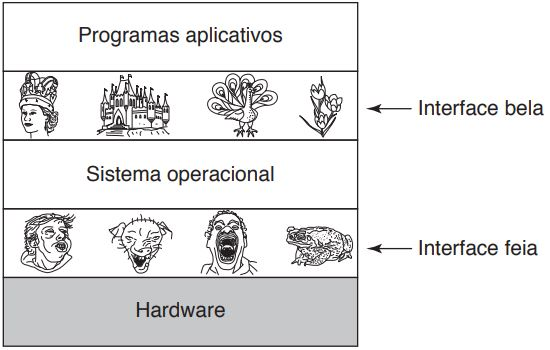
\includegraphics [scale=0.7,]{img/so_tanembaum.JPG}}
     \end{frame}
     \label{fig:so_abstracoes}
     \source{Retirado de \cite{so_tanembaum}.}
 \end{figure}

\subsection{Sistemas Operacionais Mobile}

Os SO mobile levam o mesmo conceitos que um SO tradicional, porém são aplicados em dispositivos móveis, como \textit{smartphones} e \textit{tablets}. Levam destaque, hoje, os aparelhos com suporte a \textit{touchscreen} e sem nenhum ou com poucos botões físicos. Os principais SO mobile, atualmente, são o Android, desenvolvido pela Google, e o Ios, que é propriedade da Apple. 

O Android é um sistema operacional projetado para executar em dispositivos móveis e é baseado no kernel Linux, de forma a introduzir alguns conceitos para o próprio kernel do Linux, usando a maioria dos mecanismos clássicos do Linux como processos, IDs de usuário, memória virtual, sistemas de arquivos e escalonamento, porém muitas vezes de maneira bem diferente da maneira para qual foram projetados. \citep{so_tanembaum}. 

A figura \ref{fig:so_arq_dev_android} exibe a pilha de software do android para exemplificar as camadas do sistema operacional. No nível mais baixo há o gerenciamento de energia, sobreposto por um kernel linux com seus drivers. Acima do kernel linux existe a camada de abstração de hardware, seguida pelas camadas de biblioteca de linguagem Android nativa, a a qual trabalha lado a lado com as bibliotecas de C/C++ nativas. Acima dessas duas camadas localiza-se a API do Java e no nível mais alto os aplicativos instalados no aparelho.

\begin{figure}[htb]
    \caption{Pilha de software do Android}
    \centering
    \begin{frame}{
    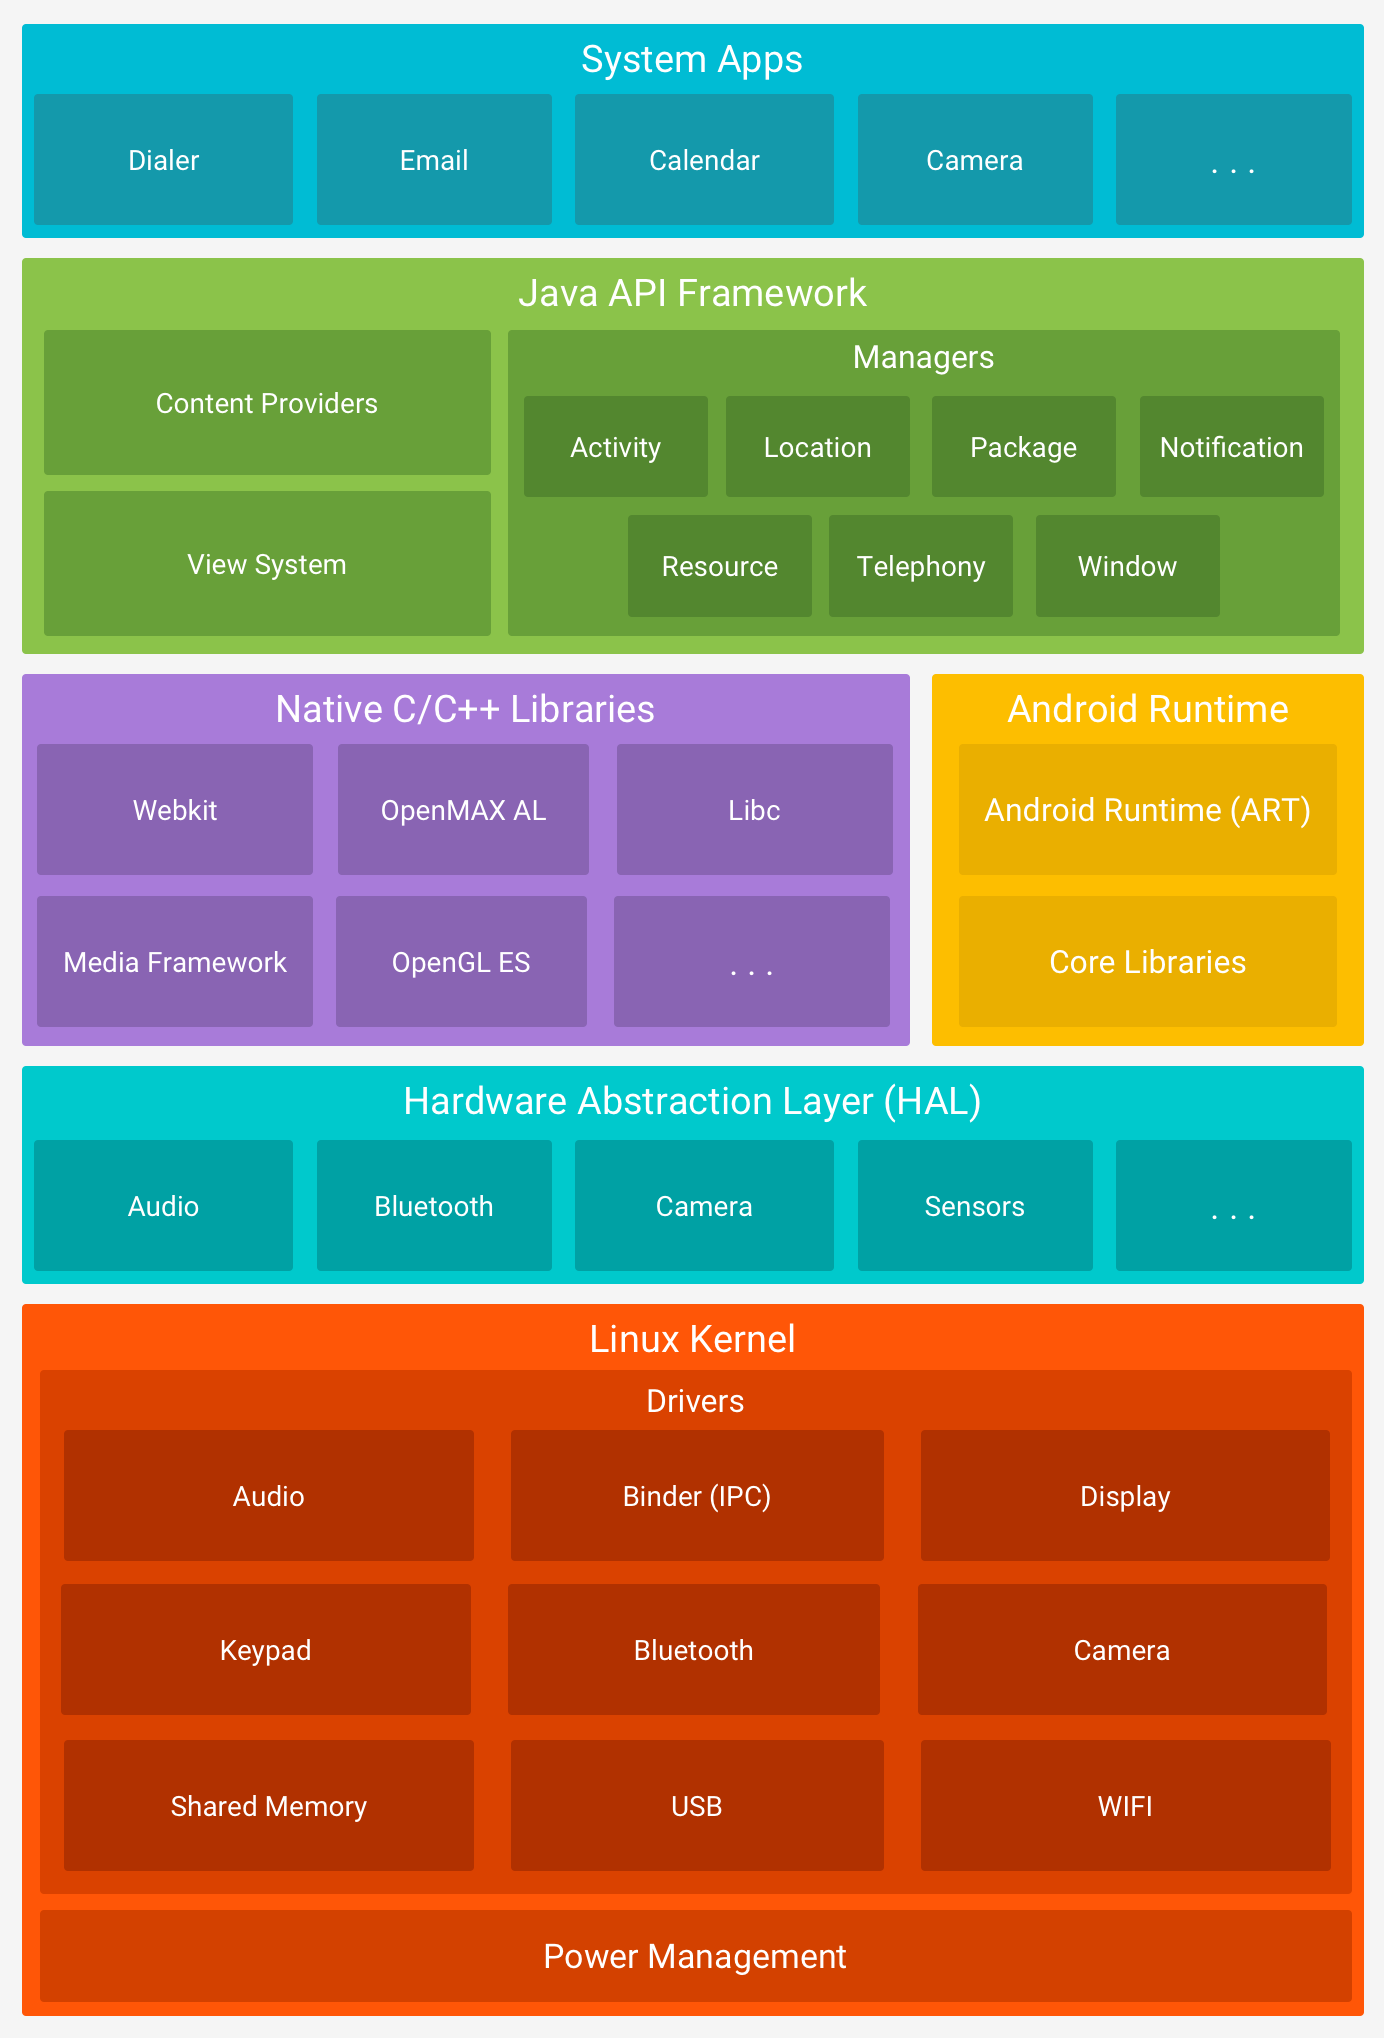
\includegraphics  [scale=0.2,]{img/arq_doc_android.png}}
    \end{frame}
    \label{fig:so_arq_dev_android}
    \source{Retirado de \cite{so_tanembaum}.}
\end{figure}

\newpage

\subsection{Arquitetura de Serviços Mobile}
A Figura \ref{fig:so_arq_android} ilustra a estrutura de processo básica do Android. Em primeiro lugar após o núcleo é o processo \textit{init},o qual gera uma série de processos de \textit{daemon} de baixo nível. Um deles é \textit{zygote}, que é a raiz dos processos de linguagem Java de nível mais alto. O \textit{init} do Android não executa um \textit{shell} da maneira tradicional, já que um dispositivo de Android típico não tem um console local para o acesso do \textit{shell}. Em vez disso, o processo \textit{daemon adbd} executa por conexões remotas que por sua vez  solicitam acesso ao \textit{shell}, criando processos do \textit{shell} para elas conforme a necessidade.

Tendo em vista que a maior parte do Android é escrita na linguagem Java, o \textit{daemon} \textit{zygote} e os processos que ele inicializa são centrais para o sistema. O primeiro processo \textit{zygote} sempre inicia e é chamado de \textit{system\_server} (serviço de sistema), que contém todos os serviços de base do sistema operacional. Partes fundamentais dele são o gerenciador de energia, gerenciador de pacotes, gerenciador de janelas e gerenciador de atividades.
Outros processos serão criados a partir de \textit{zygote} conforme a necessidade.
 
Alguns desses são processos persistentes que fazem parte do sistema operacional básico, como a pilha de telefonia no processo do telefone, que deve permanecer sempre executando. Processos de aplicativos adicionais serão criados e parados conforme a necessidade enquanto o sistema estiver executando.  

%explicar melhor essa figura
 \begin{figure}[htb]
     \caption{Hierarquia de Processos do Android}
     \centering
     \begin{frame}{
     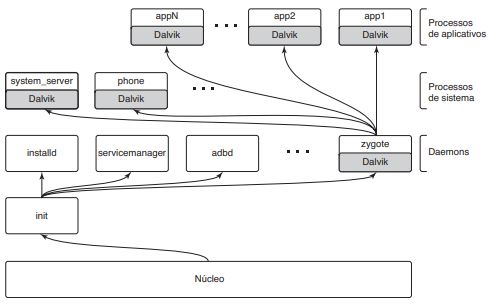
\includegraphics [scale = 1]{img/arquiteturaandroid_tanembaum.JPG}}
     \end{frame}
     \label{fig:so_arq_android}
     \source{Retirado de \cite{so_tanembaum}.}
 \end{figure}

\newpage

\subsection{Linguagem de programação}
Abordando conceitos da cadeira de "Linguagem de Programação III", se faz necessário definir a mesma. Linguagem de programação pode ser definida como uma notação formal e específica para descrever algoritmos para serem executados. Uma linguagem de programação tem dois componentes, sendo esses a Sintaxe e a Semântica. A sintaxe é um conjunto de regras que especificam a composição dos  programas a partir de caracteres. Enquanto isso, as regras de semântica devem especificar o valor de objetos inseridos nos programas \citep{apostila_lp}. 
   
\subsubsection{Dart}

Dart é uma linguagem de programação \textit{open-source} de alto nível desenvolvida pelo Google para desenvolvimento web, criada principalmente com o objetivo de facilitar a criação de aplicações web que acabam sendo muito complexas se feitas a partir dos meios tradicionais, como em linguagens de marcação \citep{dart_walratb_ladd_2012}.% https://dart.dev/mobile  %     [o que é o flutter]

\subsubsection{Flutter}
O Flutter é um framework de desenvolvimento criado pela google para o desenvolvimento de aplicativos mobile híbridos entre Ios E Android. O principal foco do Flutter é tornar o desenvolvimento o mais fácil e produtivo possível, tanto que introduz recursos tais como o \textit{Stateful Hot Reload}, função que permite carregar as alterações para o dispositivo ou emulador sendo usado para visualizar o produto sem precisar compilar todo o aplicativo a cada alteração. Também faz uso de componentes gráficos chamados \textit{Widgets}, os quais também se encontram em vários catálogos \citep{flutter_guide_2019}.

Os Widgets são basicamente componentes de inteface gráfica para o usuário, sendo podem estar organizados em blocos, linhas e colunas. Ao invés de separar as propriedades de componentes em várias \textit{views}, e outras páginas, o flutter apresenta apenas um objeto de modelo, o widget. Os widgets carregam por padrão os estilos \textit{Material}, padrão comum usado em aplicações Android, e \textit{Cupertino}, usado para Ios.

De acordo própria página de visão geral dos aspectos técnicos do Flutter, a mesma diz que o framework é um SDK para criação de aplicativos Android e Ios de alta performance a partir de um único código \citep{tec_ov_flutter}.

A Figura \ref{fig:flutter_layers} ilustra em camadas a base de funcionamento do Flutter. A figura divide em três camadas principais, sendo essas o próprio framework feito com Dart, a Engine, que no caso pode ser o Android Studio, e por último em mais baixo nível a plataforma específica do usuário, cada camada com suas subcamadas.

\begin{figure}[htb]
    \caption{Camadas do Flutter}
    \centering
    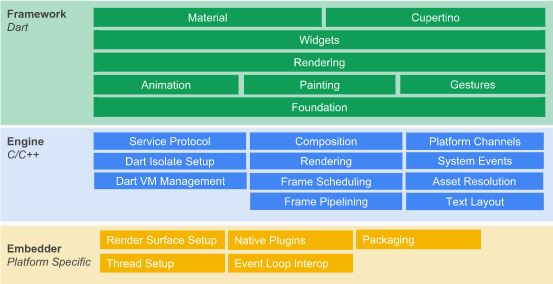
\includegraphics [scale=1.05,]{img/flutter_layers.JPG}
    \label{fig:flutter_layers}
    \source{Adaptado de \cite{tec_ov_flutter}.}
\end{figure}

\newpage

\subsection{Bancos de dados}
Por definição, um banco de dados é um agrupamento de dados que podem ser estabelecidos como o valor de representatividade de algo na vida real. A capacidade dos bancos de dados descende de um corpo de conhecimento e tecnologia que se desenvolveu ao longo de várias décadas e é representado em um software especializado chamado sistema de gerenciamento de banco de dados, ou sistema de banco de dados. Um SGBD provém acesso para criação, manutenção e afins realizados na estrutura e/ou dados inseridos no banco \citep{sbd_korth_silberchatz}.

O sistema de banco de dados é basicamente um sistema de manutenção de registros por computador - ou seja, um sistema cujo objetivo global é manter as informações e torná-las disponíveis quando solicitadas \citep{isbd_cjdate}.

Um banco de dados é uma ferramenta criada com a finalidade de gerenciar dados através de um computador, de forma que os dados nele armazenados mantenham estas informações acessíveis quando necessárias. A manipulação de um banco de dados inclui funções como consulta para recuperar dados específicos, alteração dos dados conforme a demanda e a geração de relatórios com base nos dados gravados \citep{sbd_elmasri_navathe_2011}. 

Os bancos de dados podem ser construídos a partir de um modelo relacional, embasado em um modelo entidade-relacionamento ou também podem ser bancos não relacionais. Nos bancos relacionais, as relações podem ser representadas através de um modelo de tabelas com linhas e colunas, onde as linhas representam um conjunto de valores e as colunas representam qual valor está representado.

\subsubsection{Bancos de dados não relacionais}
No contexto atual, onde um grande volume de dados é gerado a todo momento por diversas aplicações, como redes sociais, há uma grande necessidade para armazenamento e consulta de dados não estruturados, assim havendo um incentivo para o surgimento de novos paradigmas e tecnologias como uma nova categoria de banco de dados, chamada NoSQL (Not Only SQL). Essa tecnologia foi proposta com o objetivo de atender aos requisitos de gerenciamento de grandes volumes de dados, semi-estruturados ou não estruturados, que necessitam de alta disponibilidade e escalabilidade \citep{loscio_oliveira_pontes_nosql_2015}.

Em sua maioria, bancos NoSQL são escritos em JSON, conforme o código 1, adaptado da documentação do Firebase:
\begin{lstlisting}[numbers=left, language=Java, style=mycode, caption={Exemplo de modelagem JSON em Firebase.}, label={lst:firebase-code}]
{
  "usuarios": {
    "jpaulo": {
      "name": "Paulo Jaime",
      "contacts": { "edu": true },
    },
    "edu": { ... },
    "maia": { ... }
  }
}
\end{lstlisting}
\source{Adaptado da documentação do \citet{firebase_docs}.}
\justifying\setlength{\parindent}{1,25cm} 

\subsubsection{Bancos de dados em tempo real}

Sistemas em tempo real podem ser definidos como sistemas para funcionar em um tempo definido. Ou seja, executar certas tarefas com certas restrições de tempo. Portanto, a noção de correção de um sistema em tempo real depende da correção lógica dos resultados produzidos, bem como do momento em que esses resultados são produzidos \citep{realtime_db}.

Um banco de dados em tempo real é simplesmente a integração de um SGBD convencional com um Sistema em Tempo Real. Então, um SGBDTR, além de ser capaz de processar transações e ter a obrigação garantir a integridade e disponibilidade dos dados armazenados, deve trabalhar em tempo real para obedecer as regras de tempo, com as impostas aos sistemas em tempo real. As principais características de um SGBDTR contemplam a noção de dados temporalmente consistentes, e a habilidade para definir restrições temporais às transações \citep{mod_sgbdtr}. 

Ainda conforme dizem \cite{mod_sgbdtr}, observa-se casos em que há restrições temporais que quando impostas às transações precisam ser concluídas com o objetivo de manter a consistência temporal dos dados, ou seja, evitar com que atualizações dessincronizadas possam prejudicar a integridade dos dados. 

\subsubsection{Firebase}
O Firebase é um serviço da \textit{Google Cloud Platform} para prover BaaS e armazenamento de dados, além de oferecer suporte para autenticação de usuários. Quando há integração de um aplicativo com o Firebase, não há necessidade de digitar código back-end ou se preocupar com a estrutura dessa parte do programa \citep{firebase_cheng}.

O \textit{Realtime Database}  do Firebase é um banco de dados não relacional (NoSQL) que permite a distribuição de conteúdos multiplataforma  e com a possibilidade de trabalho offline. Com o Realtime Database não se faz necessária a criação e configuração de servidores ou APIs. É ótimo para validar ideias de apps e soluções web pois não requer manutenção de infra-estrutura \citep{realtime_firebase}.

\pagebreak
A estrutura do banco de dados em firebase se dá por um objeto JSON em hierarquia de árvore, essa estrutura é capaz de suportar diversos tipos de dados. A figura 4 é um exemplo de banco para um app de comércio eletrônico, onde há a produtos e clientes com suas propriedades \citep{firebase_cheng}. 

O Firebase Authentication fornece serviços de back-end e SDKs prontos para autenticar usuários em aplicativos. É oferecido suporte à autenticação através de senhas, números de telefone e até mesmo provedores como Google, Facebook, Twitter entre outros.

Para conectar um usuário a um app, primeiro deve-se ter as credenciais de autenticação do usuário, podendo ser o endereço de e-mail e a senha do usuário ou até mesmo um token de acesso do OAuth de um provedor de identidade federado. Então, são essas credenciais são enviadas para o SDK do Firebase Authentication, onde o back-end faz a  verificação e retorna-se uma resposta ao cliente \citep{firebase_docs}.

Após fazer login, se tem acesso a informações básicas do perfil do usuário e também a capacidade de controlar o acesso do mesmo aos dados armazenados em outros produtos do Firebase. É possível também usar o token de autenticação fornecido para verificar a identidade dos usuários nos seus próprios serviços de back-end \citep{firebase_docs}.

Para o armazenamento de arquivos no firebase usa-se a função de \textit{Cloud Storage}. Com os SDKs do Firebase para Cloud Storage, é permitido fazer \textit{upload} e \textit{download} de arquivos nos aplicativos associados ao Firebase, independentemente da qualidade da rede. Os arquivos são armazenados em um repositório do GCP e são acessados por meio do Firebase. Isso permite executar processos no servidor como filtragem de imagens, vídeo ou outro tipo de documento \citep{firebase_docs}. 

Além disso, o firebase dispõe de uma ferramenta para facilitar o envio de notificações ao usuário através do app, o Firebase Cloud Messaging (FCM). O FCM é uma solução para o envio de mensagens entre plataformas que permite o envio de notificações. A equipe de desenvolvimento pode enviar mensagens de notificação para promover novas interações ou até mesmo tentar influenciar a retenção de usuários. Para casos de uso como mensagens instantâneas, uma mensagem pode transferir um payload de até 4 KB para um app cliente \citep{firebase_docs}.

\subsubsection{GCP - Google Cloud Platform}
O GCP consiste em uma plataforma de acesso a ativos de hardware e software da Google, sendo que esses ativos estão distribuídos em diversos centros da Google pelo mundo. As regiões se dividem em EUA, Europa Ocidental e leste da Ásia, sendo que as mesmas se subdividem em zonas, e a zona, por sua vez, é identificada através de uma nomenclatura que combina um identificador de letra com o nome da região. Como por exemplo, a zona a na região do Leste da Ásia se chama \textit{asia-east1-a}. A distribuição de recursos oferece  vantagens como redundância em caso de falha e também latência reduzida localizando recursos mais próximos de cada cliente, bem como introduz regras sobre como recursos podem ser usados juntos \citep{gcp_2019} .

\subsubsection{Projetos GCP e Firebase}
Para usar ou alocar quaisquer recursos do GCP, é necessário um projeto. Um projeto pode ser pensado como a entidade organizadora do que se está construindo. Um projeto no GCP é feito das configurações, permissões e de outros metadados que descrevem os aplicativos. Os recursos alocados dentro de um único projeto podem funcionar juntos, por exemplo, comunicando-se por meio de uma rede interna. Os recursos usados por cada projeto sempre se mantém separados por limites de projeto entre si, para conectar os mesmos só é possível através de uma rede de internet \citep{gcp_2019}.

Ao criar um novo projeto no Console do Firebase, na verdade está sendo criado um projeto do GCP. É possível fazer a analogia de  um projeto do GCP como um \textit{container} virtual para dados, código, configurações e serviços. Então, um projeto do Firebase é um projeto GCP com configurações e serviços específicos do Firebase. Da mesma forma, também é possível criar um projeto do primeiramente no GCP para depois adicionar o Firebase ao mesmo \citep{firebase_docs}.

Ainda de acordo com a documentação do \citeauthor{firebase_docs}, identifica-se alguns pontos para corroborrar o fato de um projeto do Firebase ser um projeto do GCP, estes são:

\begin{itemize}
    \item Os projetos que aparecem no console do Firebase também aparecem no Console do GCP e no Console de APIs do Google.
    \item O faturamento e as permissões para projetos são compartilhados entre o Firebase e o GCP.
    \item Os identificadores exclusivos de um projeto (como project ID) são compartilhados entre o Firebase e o GCP.
    \itemé possível usar produtos e APIs do Firebase e do GCP no seu projeto.
    \item A exclusão de um projeto o exclui no Firebase e no GCP.
\end{itemize}

\begin{figure}[htb]
     \caption{Visão geral console do projeto no Firebase}
     \centering
     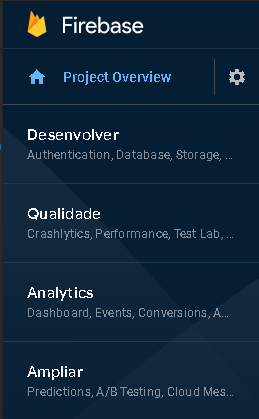
\includegraphics {img/firebase_console.PNG}
     \label{fig:firebase_console}
     \source{Adaptado de \cite{firebase_docs}}   
 \end{figure}
	
Em relação a custos, o Firebase se divide em três planos: \textit{Spark}, \textit{Flame} e \textit{Blaze}, conforme a Figura \ref{fig:firebase_precos}. Como benefício padrão de todos os planos, estão incluídas as funções de análises, notificações, relatórios de erros, suporte e alguns outros.

O \textit{Spark} é o plano gratuito, o mesmo permite o uso limitado das funções de \textit{database, storage, functions, phone auth, hosting} e \textit{test lab}. o Flame é um plano de valor fixo, no valor de US\$ 25,00 por mês e além das funcionalidades do plano \textit{spark}, o flame possui maior espaço disponível no \textit{database} e suporte conexões para o \textit{functions}. Por último, o Blaze, um plano que é pago pela utilização e pode incluir todas as funções do Firebase ao projeto.

\begin{figure}[htb]
    \caption{Planos de preços no Firebase}
    \centering
    \begin{frame}{
    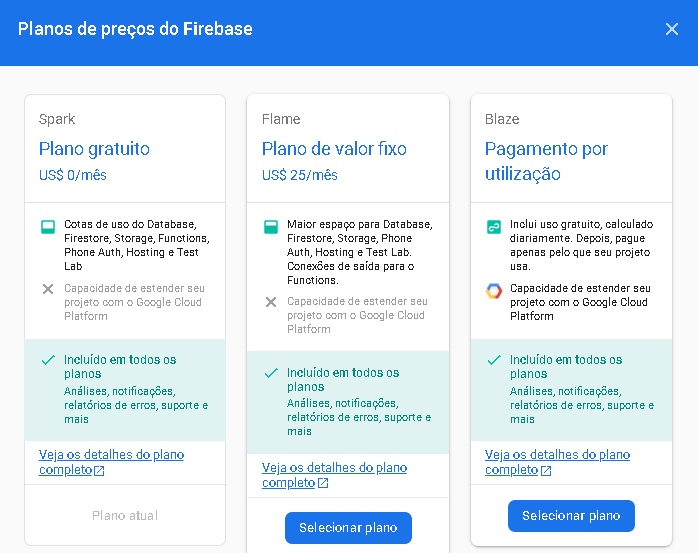
\includegraphics [scale = 0.825]{img/firebase_precos.PNG} }
    \end{frame}
    \label{fig:firebase_precos}
    \source{Retirado de \cite{firebase_docs}}
\end{figure}
% Chapter 3
\chapter{Análise e discussão de resultados}\label{chap:Results}

Ao decorrer deste capítulo são apresentados, respectivamente, a identificação das partes interessadas no aplicativo seguido de suas necessidades e problemas, a análise do sistema com os diagramas de processo, caso de uso e diagramas de classe. Em seguida é apresentada a proposta de aplicativo, o protótipo, os resultados esperados e as áreas que serão afetadas pelo app.

\section{Situação Atual}
O aplicativo será desenvolvido baseado no ambiente da empresa Abase Sistemas e Soluções LTDA, uma empresa de software localizada na cidade de Três de Maio - RS e com sua fundação realizada em 1989. Atualmente a Abase tem duas áreas de trabalho bem definidas. Uma das áreas desenvolve sistemas para a gestão pública, tendo como clientes a maior parte das prefeituras da região, e a outra área trabalha no desenvolvimento de um ERP para empresas privadas, tendo como objetivo fornecer as melhores inovações tecnológicas através de seus softwares aplicativos integrados. 

Ao conversar com o responsável de infraestrutura da empresa, foi possível observar que atualmente não há controle para os chamados internos de infraestrutura de TI em específico, só há registros dos chamados de requisição de serviços de suporte para desenvolvimento e vice-versa em para chamados de clientes. Quando há necessidade de solicitar algo para a infraestrutura, usa-se telefone, \textit{Skype}, \textit{Whatsapp} ou até mesmo indo pessoalmente até a sala do responsável e descrevendo o problema. Ou seja, não há uma forma padrão para criar ou responder chamados, o que de acaba prejudicando o gerenciamento de processos.

Os chamados que são registrados, são feitos através do sistema de atendimento ao cliente de uma empresa terceirizada tendo a empresa cadastrada como um cliente e os funcionários como usuários. O grande problema sempre ao ter um sistema para gerenciar os chamados é convencer o usuário a usar, para adotar o uso se faz necessário exigir o cadastro de uma tarefa no sistema de chamados para a mesma ser executada. Caso seja exigida a execução de um serviço, o mesmo não poderia ser feito sem ter um chamado associado. 

De acordo com as próprias palavras do responsável, o fato de ter um aplicativo como o proposto, poderia permitir que um chamado fosse fechado assim que uma tarefa foi executada, em qualquer lugar. Por exemplo; ao trocar o teclado de um usuário que já havia feito o pedido, o responsável pela troca poderia finalizar o chamado no local, sem ter a necessidade de retornar ao seu computador para faze-lo.

\section{Especificação dos requisitos e processos}
% Deve descrever o que se deseja do sistema a ser desenvolvido. Não são necessários  modelos gráficos neste item. Os principais subitens da especificação são:
Ao dispor a contextualização da situação atual do processo na empresa e também dos objetivos e problema propostos, é possível escalar as funcionalidades que se desejam no aplicativo. 

O app está sendo desenvolvido tendo como foco padronizar a forma de gerar chamados de suporte de TI internamente na empresa. Em geral, o aplicativo deve permitir a abertura de chamados, o monitoramento de chamados abertos, fechar chamados, classificar um chamado como pausado, classificar um chamado como aberto, finalizar chamado aberto e também permitir a visualização dos detalhes de um chamado independente do status.


\subsection{Requisitos funcionais} %casos de uso e funcionalidades
Como requisitos funcionais podem ser identificados os casos de: criar chamado, atender chamado, pausar chamado,  retomar atendimento de chamado pausado, finalizar chamado e ver detalhes de chamado. Os requisitos funcionais são descrições específicas dos casos de uso que são aplicados as regras de negócio, conforme o diagrama de caso de uso, ilustrado na Figura \ref{fig:diagrama_caso_de_uso}.

\begin{figure}[htb]
     \caption{Diagrama de caso de uso}
     \centering
     \begin{frame}{
     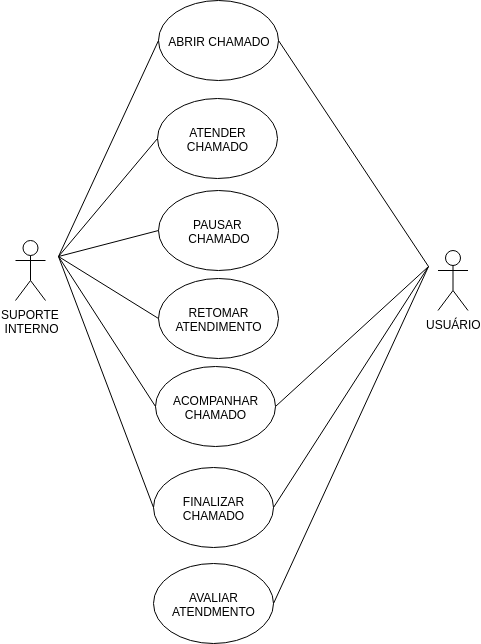
\includegraphics [scale = 0.7]{img/Diagramas/diagrama_caso_de_uso.png}}
     \end{frame}
     \label{fig:diagrama_caso_de_uso}
 \end{figure}
\newpage
Portanto, a partir da ilustração do diagrama, é possível identificar os requisitos funcionais do aplicativo para  então descrever os mesmos. Os requisitos identificados são Criar Chamado, Atender chamado, pausar chamado, retomar atendimento, finalizar chamado e avaliar atendimento, os quais estão respectivamente descritos como:\\

\noindent\fbox{
    \parbox{\textwidth}{
        \small\textbf{RF1 - Criar Chamado} \smallskip\hrule\ \\
        \small\textbf{Descrição:} A criação de um chamado é o início do fluxo do chamado no sistema. Após o chamado ser criado, o mesmo entra em \textit{workflow} onde é possível visualizar o status do chamado conforme o andamento do mesmo e então interagir com os cartões de chamado.\\
        \small\textbf{Ator:} Atendente ou Usuário.\\
        \small\textbf{Entrada:} É necessário informar um título, a classificação e a descrição do incidente, podendo também anexar uma imagem. A classificação pode ser Hardware, software, rede, impressora, ou telefonia. Além da classificação o usuário deve informar o tipo do chamado, que pode ser Incidente, Requisição de Serviço ou Melhoria.\\ 
        \small\textbf{Saída Principal:} após clicar no botão de concluir, exibir uma mensagem de confirmação.\\
        \small\textbf{Saída alternativa:} caso campos obrigatórios não sejam preenchidos, notificar nos campos através dos validadores.
        \\
    }
}

\noindent\fbox{
	    \parbox{\textwidth}{
	        \small\textbf{RF2 - Atender Chamado} \smallskip\hrule\ \\
	        \small\smallskip\textbf{Descrição:} Para iniciar o atendimento, o chamado já \smalldeve ter sido criado anteriormente e deve estar com status "em espera". Essa função tem como objetivo destacar o chamado como estando em atendimento. \\
	        \small\textbf{Ator:} Atendente. \\
	        \small\textbf{Entrada:} Como entrada pode ser considerado o chamado em si e também a confirmação no botão de atender, inserido no cartão do chamado\\
	        \small\textbf{Saída Principal:} O cartão do chamado deve ir para aba "em atendimento".\\
	    }
	}

\noindent\fbox{
	    \parbox{\textwidth}{
	        \small\textbf{RF3 - Priorizar Chamado} \smallskip\hrule\ \\
	        \small\smallskip\textbf{Descrição:} Ao atender um chamado, o atendente deve classificar o mesmo em relação a seu nível de prioridade. \\
	        \small\textbf{Ator:} Atendente. \\
	        \small\textbf{Entrada:}O chamado deve ser classificado de acordo com sua prioridade, podendo ser Baixo, Médio, Alto ou Crítico.\\
	        \small\textbf{Saída Principal:} O cartão do chamado deve apresentar um ícone identificador para cada uma destas situações.\\
	    }
	}
	
\noindent\fbox{
	    \parbox{\textwidth}{
	        \small\textbf{RF4 - Ordenar Lista de Chamados} \smallskip\hrule\ \\
	        \small\smallskip\textbf{Descrição:} Ordena a lista de chamados de acordo com sua prioridade ou data de abertura do chamado. \\
	        \small\textbf{Ator:} Atendente ou Usuário. \\
	        \small\textbf{Entrada:}Como entrada pode ser considerado o filtro utilizado.\\
	        \small\textbf{Saída Principal:} Deve retornar a listagem seguindo o ordenamento definido pelo Atendente ou Usuário.\\
	    }
	}

\noindent\fbox{
	    \parbox{\textwidth}{
	        \small\textbf{RF5 - Pausar Chamado} \smallskip\hrule\ \\
	        \small\smallskip\textbf{Descrição:} A função de pausar chamado refere-se a necessidade de deixar um chamado pausado depois de já ter sofrido o primeiro atendimento. Um chamado pausado diferencia-se de um chamado em espera pelo fato de que um chamado em espera não passou pelo primeiro atendimento ainda, apenas pela abertura do mesmo.  \\
	        \small\textbf{Ator:} Atendente. \\
	        \small\textbf{Entrada:}Como entrada pode ser considerado o chamado em si e também a confirmação no botão de pausar chamado. \\ 
	        \small\textbf{Saída Principal:} O cartão do chamado deve ir para aba "pausado". \\
	    }
	}

\noindent\fbox{
        \parbox{\textwidth}{
            \small\textbf{RF6 - Retomar Atendimento} \smallskip\hrule\ \\
            \small\textbf{Descrição:} A função de retomar tem por objetivo retomar o atendimento do chamado pausado.  \\
            \small\textbf{Ator:} Atendente \\
            \small\textbf{Entrada:} Como entrada pode ser considerado o chamado em si e também a confirmação no botão de "Retomar Chamado". \\
            \small\textbf{Saída Principal:} O cartão do chamado deve ir para aba "em atendimento".\\
        }
    }
    
\noindent\fbox{
    \parbox{\textwidth}{
        \small\textbf{RF7 - Acompanhar Chamado} \smallskip\hrule\ \\
        \small\textbf{Descrição:} Deve permitir tanto ao usuário quanto ao atendente de suporte visualizar detalhes acerca do chamado, independente do status em que o chamado se encontra.\\
        \small\textbf{Ator:} Atendente ou Usuário\\
        \small\textbf{Entrada:} O usuário/atendente deve selecionar o chamado que desejam consultar. \\
        \small\textbf{Saída Principal:} Exibe detalhes do chamado selecionado.\\
        \small\textbf{Saída alternativa:} Deve informar que os detalhes não puderam ser carregados.\\
    }
}

\noindent\fbox{
        \parbox{\textwidth}{
            \small\textbf{RF8 - Finalizar Chamado} \smallskip\hrule\ \\
            \small\textbf{Descrição:} Permite ao atendente finalizar o chamado, alterando o status para "Concluído".\\
            \small\textbf{Ator:} Atendente\\
            \small\textbf{Entrada:} O atendente deve marcar o chamado como "Concluído".\\
            \small\textbf{Saída Principal:} Informa que o chamado foi concluído com sucesso.\\
        }
    }
    
\noindent\fbox{
        \parbox{\textwidth}{
            \small\textbf{RF9 - Avaliar Atendimento} \smallskip\hrule\ \\
            \small\textbf{Descrição:} O usuário poderá avaliar o atendimento com notas entre 1 e 5 após o encerramento do chamado. Esta avaliação não é obrigatória. \\
            \small\textbf{Ator:} Usuário\\
            \small\textbf{Entrada:} O usuário poderá selecionar um valor entre 1 e 5 ou optar por não responder.\\ 
            \small\textbf{Saída Principal:} Informa que o atendimento foi concluído.\\
        }
    }
    
\noindent\fbox{
        \parbox{\textwidth}{
            \small\textbf{RF10 - Registro de Resolução} \smallskip\hrule\ \\
            \small\textbf{Descrição:} Ao final do atendimento, o atendente poderá registrar o que foi realizado para que a situação fosse resolvida, para que possa consultar caso tenha dúvida em futuros atendimentos. \\
            \small\textbf{Ator:} Atendente\\
            \small\textbf{Entrada:} O atendente poderá informar o que foi realizado para resolver o chamado em questão.\\ 
            \small\textbf{Saída Principal:} Informa que a resposta foi registrada.\\
        }
    }

\subsection{Requisitos não funcionais}
Os requisitos não funcionais são aqueles necessários para o funcionamento da aplicação, porém não interferem nas regras de negócio. De tal forma, foram elencados como requisitos não funcionais foram Sistema operacional Android, Conexão com Internet, Sincronização com banco de dados e Login, respectivamente descritos abaixo:

\noindent\fbox{
    \parbox{\textwidth}{
        \small\textbf{RNF1 - Sistema Operacional Android} \smallskip\hrule\ \\
        Para utilização da aplicação, o usuário deve dispor de um smartphone ou tablet que utilize o sistema operacional Android.
    }
}

\noindent\fbox{
    \parbox{\textwidth}{
        \small\textbf{RNF2 - Conexão com Internet} \smallskip\hrule\ \\
        A Conexão com a internet se faz necessária para sincronizar os dados com o serviço do Firebase. O sistema deve ter implementado um modo \textit{offline first} para gravar chamados ou eventuais mudanças nos chamados no próprio smartphone em caso de falta de conexão com a internet.
    }
}

\noindent\fbox{
    \parbox{\textwidth}{
        \small\textbf{RNF3 - Sincronização com banco de dados} \smallskip\hrule\ \\
        O sistema deve ter implementado um modo \textit{offline first} para gravar chamados ou eventuais mudanças nos chamados no armazenamento do próprio smartphone em caso de falta de conexão com a internet. Ao reconectar o dispositivo, a sincronização com o serviço do Firebase deve ser automática
    }
}

\noindent\fbox{
    \parbox{\textwidth}{
        \small\textbf{RNF4 - Login} \smallskip\hrule\ \\
        O acesso de cada usuário do app deve acontecer a partir de um login e senha único por usuário. \\
        Deve haver dois tipos de usuário, sendo um "Atendente" e outro "Usuário" 
    }
}

\section{Identificação do processo} 
Conforme demonstra a Figura \ref{fig:diagrama_processos}, o processo de atendimento se inicia com a ocorrência de algum tipo de problema para o usuário, o qual abre um chamado de suporte. Neste ponto, é permitido ao atendente do suporte atender ou finalizar este chamado, tendo atendido este chamado, ele pode ser pausado conforme necessário. Após finalização do chamado, o usuário pode optar entre avaliar o atendimento ou não. Caso deseje, poderá dar a sua avaliação através de uma pontuação entre 1 e 5.

\begin{figure}[htb]
     \caption{Diagrama de processo}
     \centering
     \begin{frame}{
         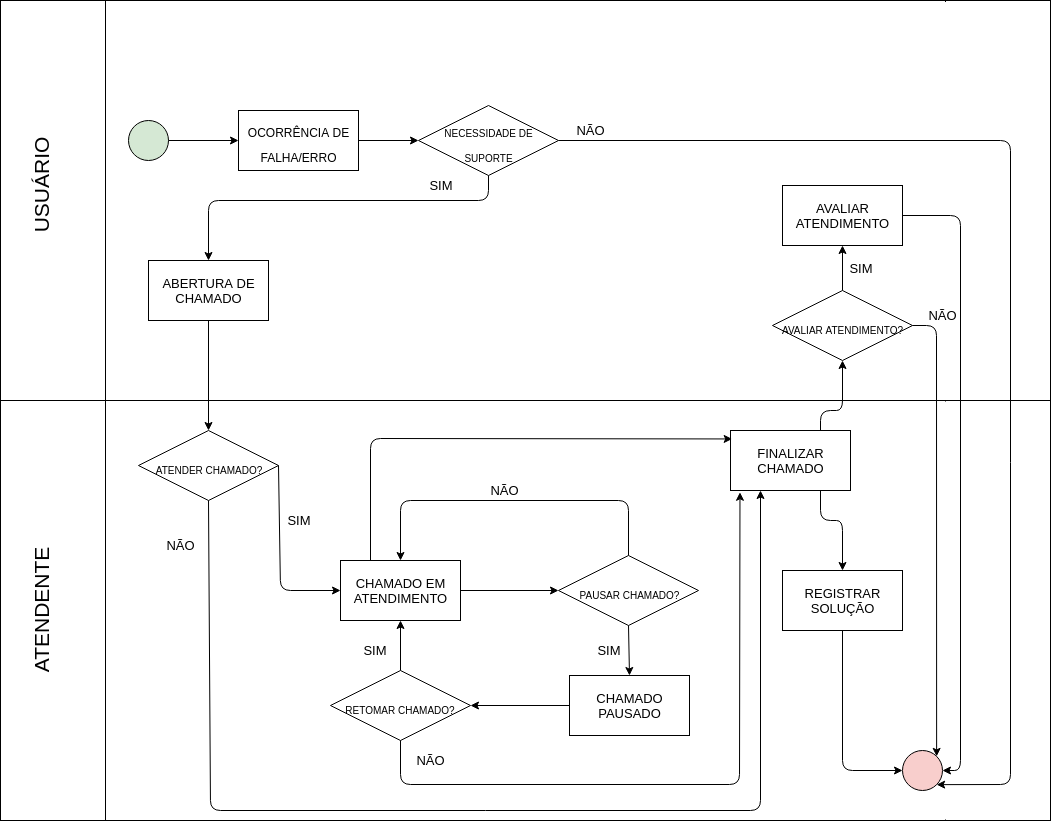
\includegraphics [scale = 0.41]{img/Diagramas/diagrama_processos.png}}
     \end{frame}
     \label{fig:diagrama_processos}
 \end{figure}
\newpage

\subsection{Diagrama de Classes}
A Figura \ref{fig:diagrama_classes} tem por objetivo identificar as classes presentes no app. O aplicativo é composto por basicamente 3 classes, sendo essas: Usuario, Chamado e Login.
A classe de usuário possui como atributos um id, nome, senha, nível de usuário e foto de perfil, tem como método direto o logout.
A classe Chamado possui os atributos de Id, titulo, descricao, prioridade, classificação e foto, e da mesma forma possui seus métodos: abrirChamado, finalizarChamado, pausarChamado, atenderChamado e avaliarChamado.


\begin{figure}[htb]
     \caption{Diagrama de classes}
     \centering
     \begin{frame}{
     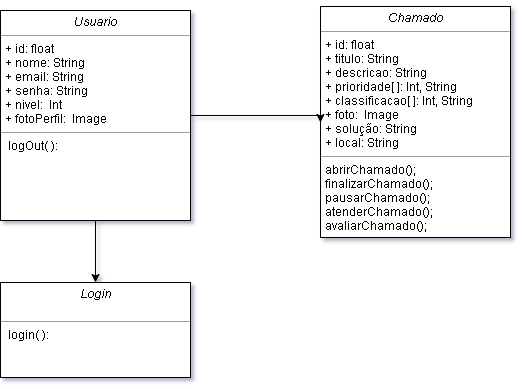
\includegraphics [scale = 0.83]{img/Diagramas/diagrama_classes.png}}
     \end{frame}
     \label{fig:diagrama_classes}
 \end{figure}
\newpage

\subsection{Resultados esperados}
Ao se atingir o prazo final para o fim do desenvolvimento, era esperado que o app desenvolvido proponha a capacidade de abrir chamados de suporte, acompanhar os chamados abertos e avaliar os chamados depois de atendidos, além de permitir que um usuário de nível atendente seja capaz de manipular o status de chamado entre "em espera", "em atendimento", "pausado" e "finalizado". O app deve rodar em smartphones com sistema operacional Android. 

Apesar de o aplicativo ser desenvolvido em uma plataforma de código híbrido, o uso em aparelhos com IOS só pode ser feito a partir do download da loja de aplicativos da Apple ou usando um computador com MacOS como ambiente de desenvolvimento, o que não se identifica como o cenário atual para desenvolvimento do aplicativo pelos acadêmicos, os mesmos somente possuem acesso a computadores com sistema operacional Windows e Linux, assim como somente smartphones Android. No entanto, devido aos fundamentos do framework Flutter, o mesmo projeto pode ser compilado em um computador com MacOS e com um aparelho IOS e funcionar da mesma maneira,  

\subsection{Áreas afetadas}
No ambiente da empresa, podem-ser afetadas principalmente a área de infraestrutura de TI, principalmente no quesito de organização das atividades do atendente. Além disso pode afetar todas as áreas da empresa que eventualmente façam pedidos para a área de infraestrutura de TI.

\section{Apresentação do aplicativo desenvolvido}
Esse capítulo aborda a apresentação do que foi desenvolvido como interface final do app. Assim como a apresentação do software em relatório, foi feita a documentação do app para o usuário, disponível no Apêndice III deste documento. 

De forma básica, o app baseia-se em uma tela principal com a visualização de 4 abas, sendo essas os status de um chamado. O protótipo do aplicativo também dispõe de uma tela de login que da acesso a tela dos chamados. 

A tela principal, além das 4 abas para mostrar os chamados em seus status, dá acesso a tela de criar chamado através do \textit{Floating Action Button} com o \textit{label} '+ Novo' e também um menu lateral como um \textit{Drawer} onde deve ser exibida as informações do usuário acessado. O login dos atendentes deve ser feito por um usuário e senha criados, até então, de forma manual através do Acesso ao Firebase, já para os demais usuários, o login deve ser a partir de uma conta google.

Também foi elaborado um resumo expandido com os resultados do trabalho para apresentações em futuros eventos. O resumo expandido pode ser encontrado no Apêndice IV deste documento.
\newpage
A Figura \ref{fig:1_login} representa a tela de login, na qual há os campos de usuário e senha com um botão para fazer o login. Ao clicar no botão de login, o app deve redirecionar para a página principal dos chamados.
\begin{figure}[htb]
     \caption{Print de tela 1 - Tela de login}
     \centering
     \begin{frame}{
     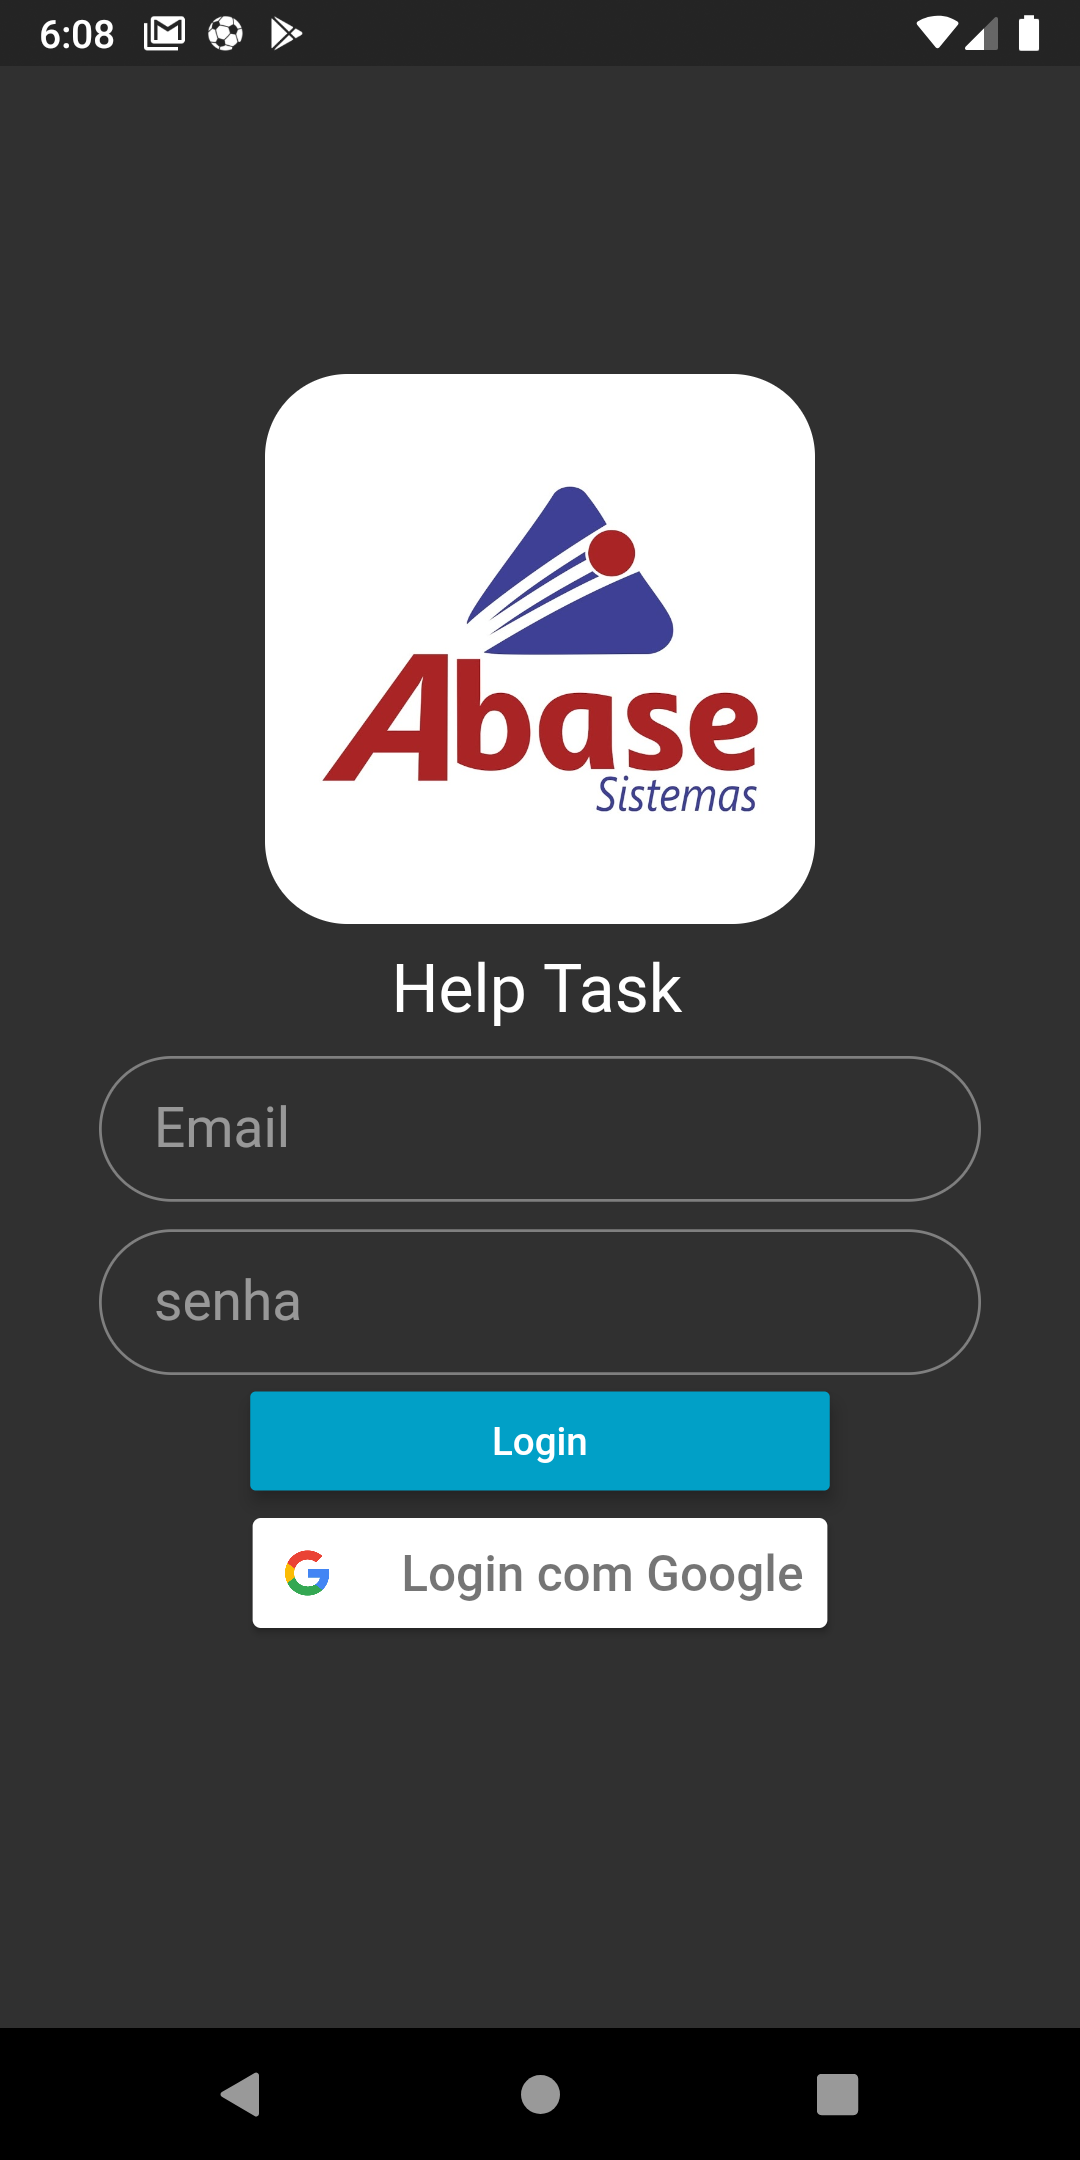
\includegraphics [scale = 0.2]{img/screenshots/1_login.png}}
     \end{frame}
     \label{fig:1_login}
 \end{figure}
\newpage

A Figura \ref{fig:2_em_espera} Representa a tela principal com a aba de chamados em espera, nessa tela são listados todos os chamados que ainda não foram atendidos, portanto os chamados podem ser atendidos ou finalizados diretamente.
\begin{figure}[htb]
     \caption{Print de tela 2 - Lista de chamados em espera}
     \centering
     \begin{frame}{
     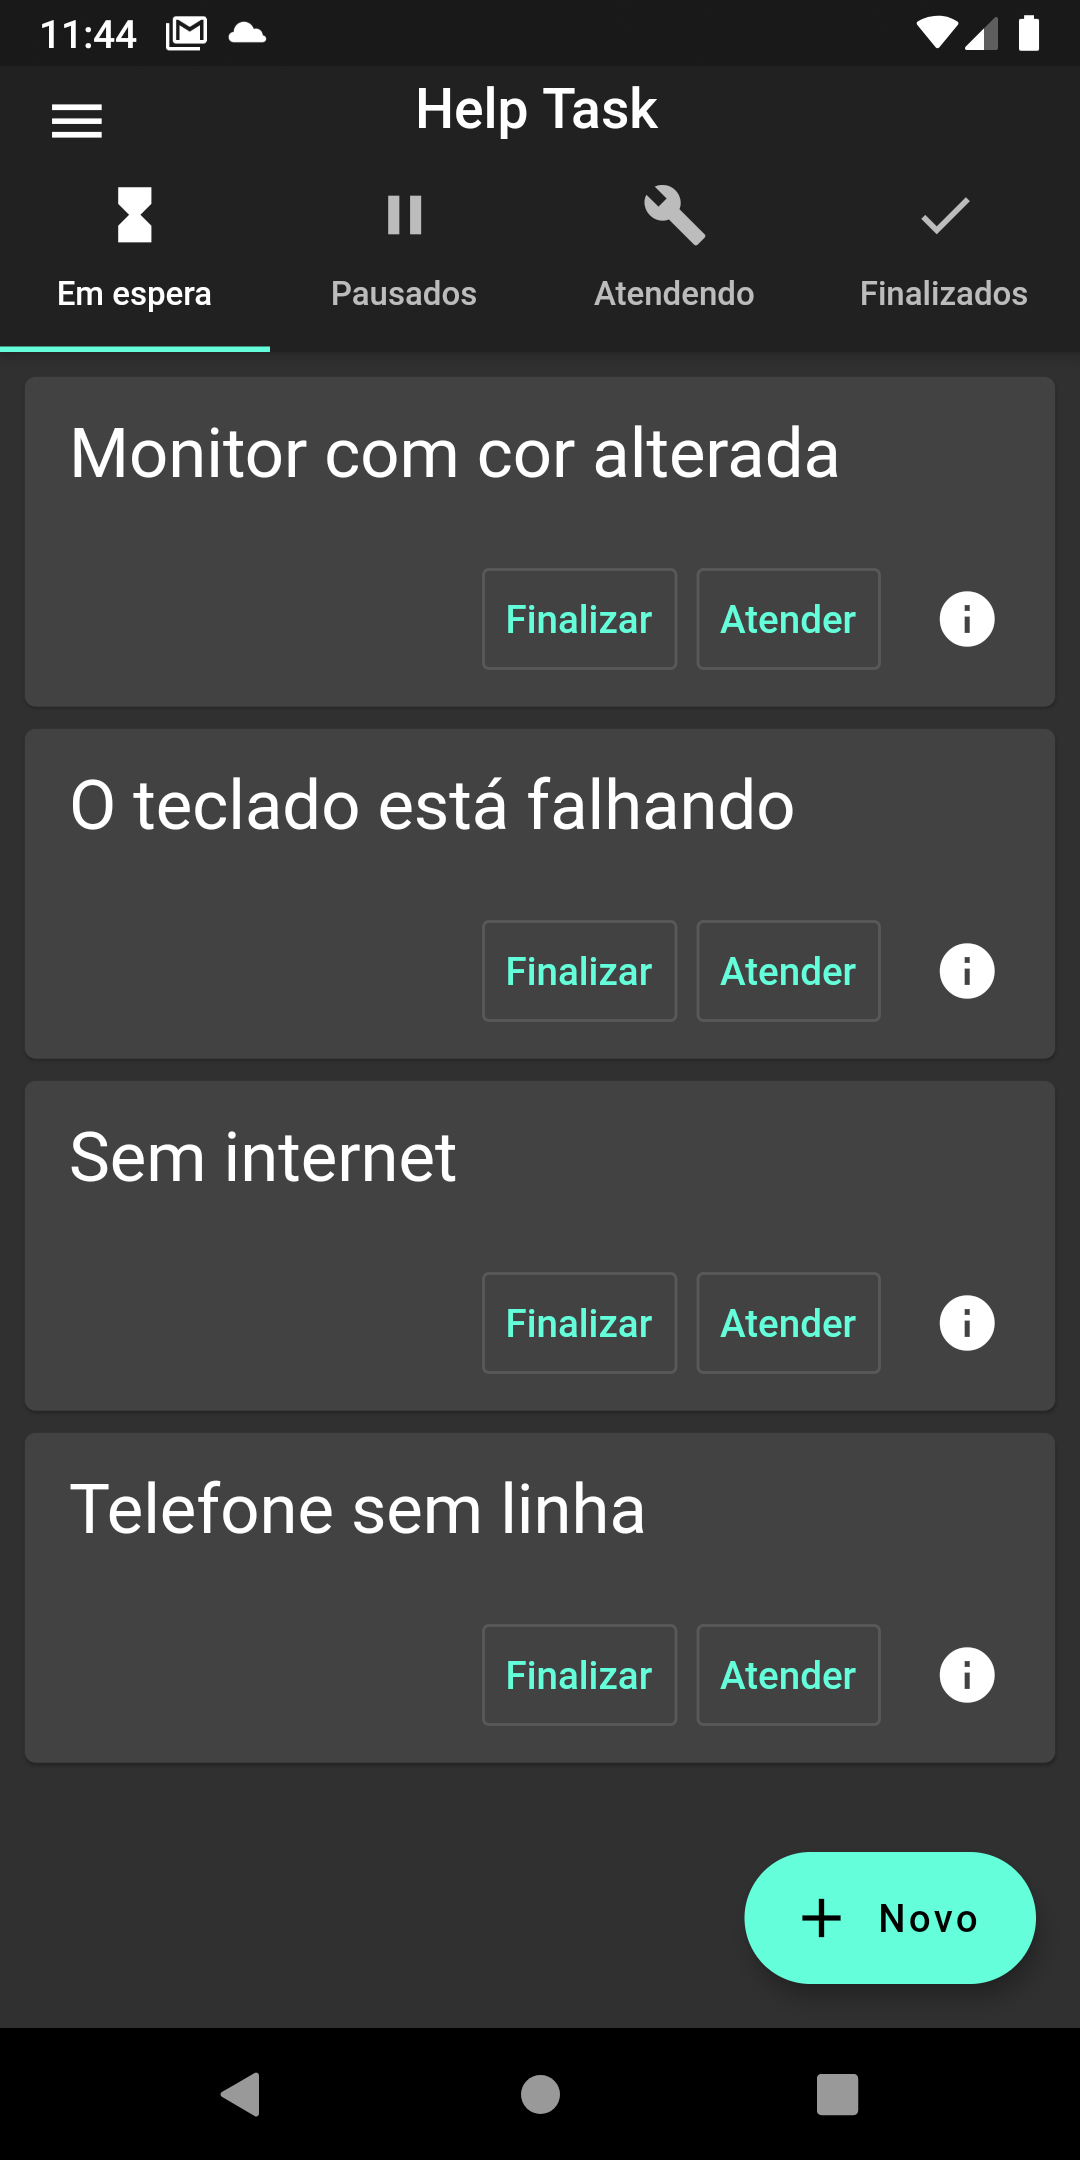
\includegraphics [scale = 0.2]{img/screenshots/2_em_espera.png}}
     \end{frame}
     \label{fig:2_em_espera}
 \end{figure}
\newpage

Na aba de chamados pausados, como mostra a Figura \ref{fig:3_pausados}, se localizam os chamados  que já foram atendidos pelo menos uma vez, nessa parte os chamados podem ser retomados para voltar a aba de atendimento.
\begin{figure}[htb]
     \caption{Print de tela 3 - Lista de chamados pausados}
     \centering
     \begin{frame}{
     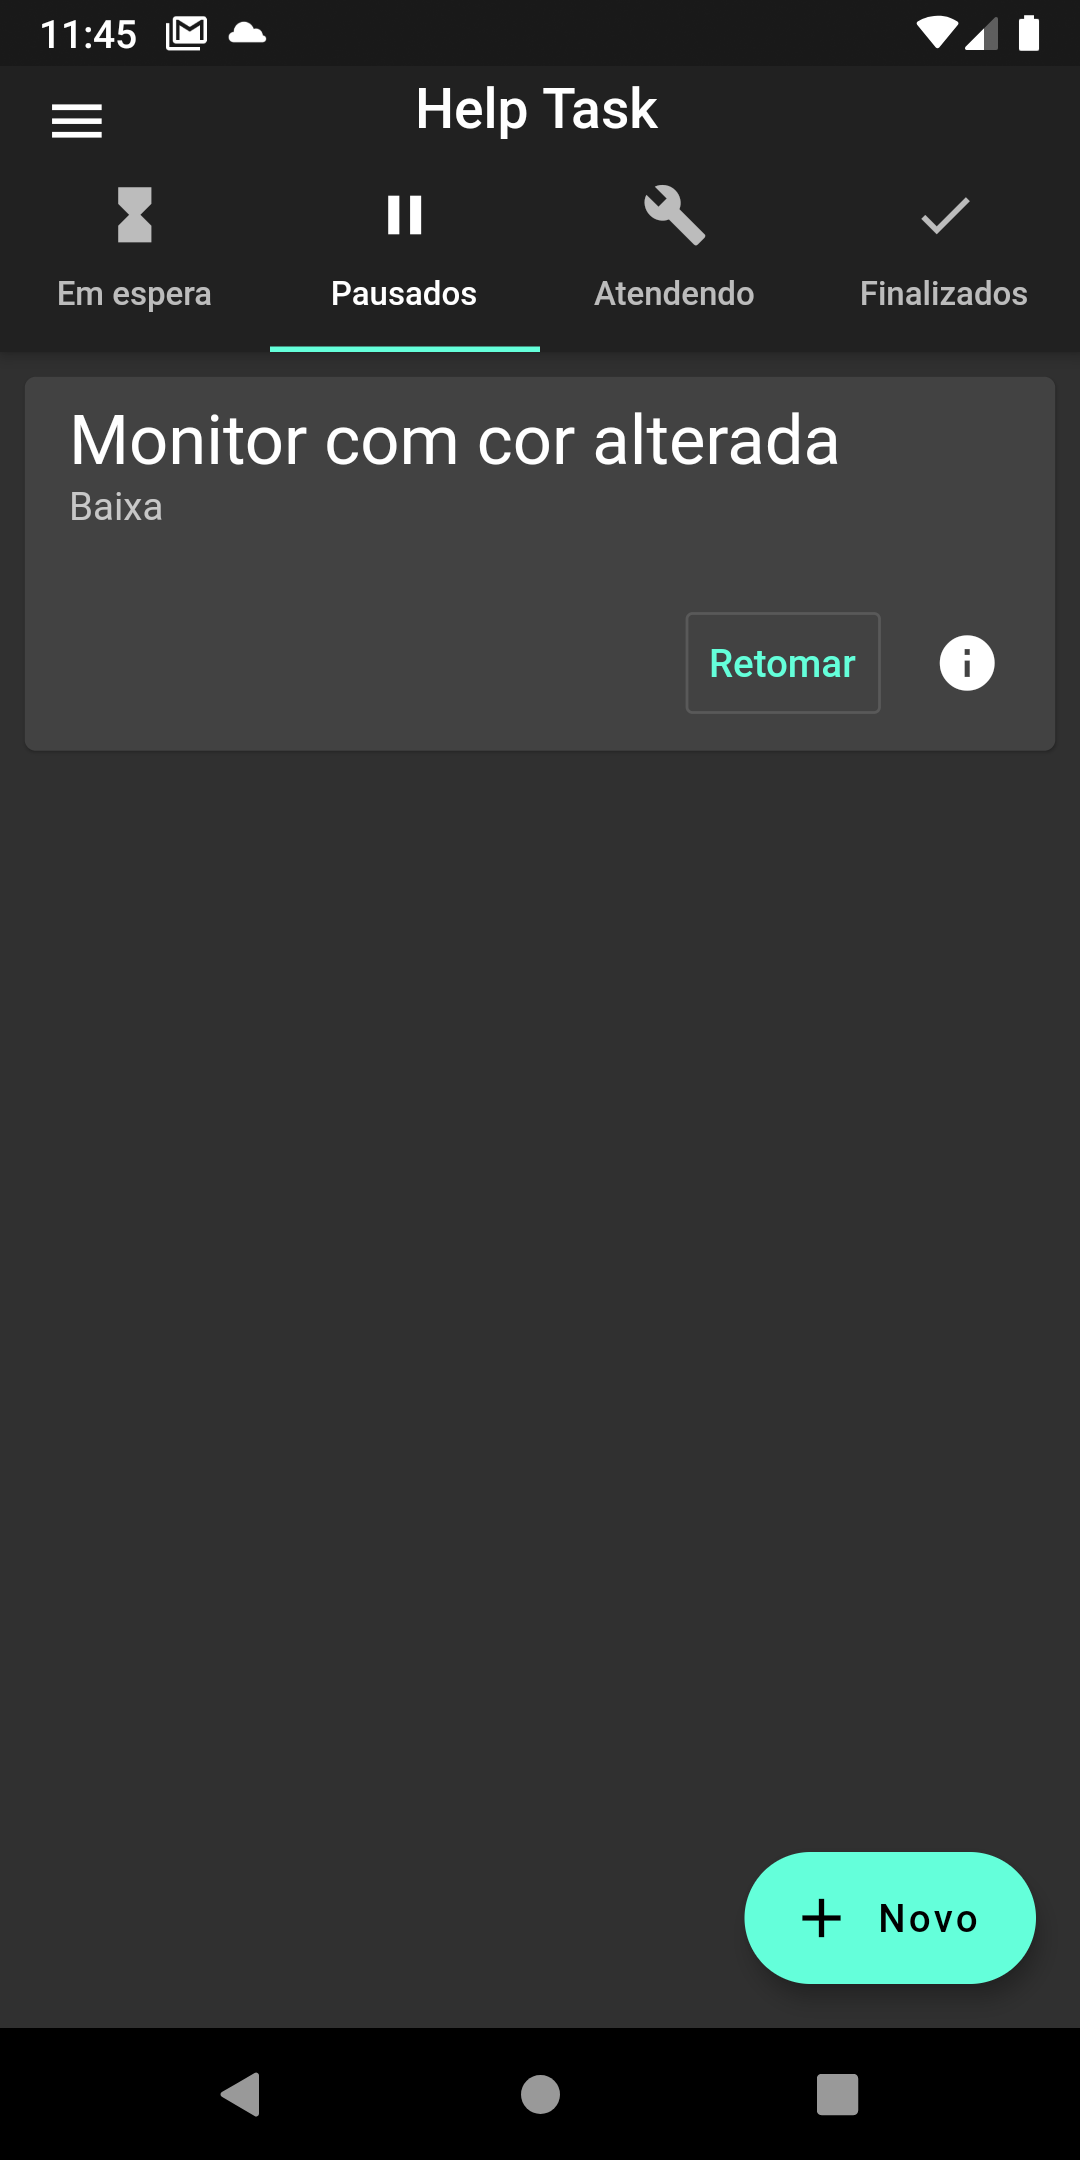
\includegraphics [scale = 0.2]{img/screenshots/3_pausados.png}}
     \end{frame}
     \label{fig:3_pausados}
 \end{figure}
\newpage

Na aba de chamados em atendimento, conforme a Figura \ref{fig:4_atendendo}, se localizam os chamados que estão sendo atendidos. Nessa parte, os chamados podem ser finalizados ou pausados. Para Finalizar um chamado o atendente deve informar uma justificativa.

\begin{figure}[htb]
     \caption{Print de tela 4 - Lista de chamados em atendimento}
     \centering
     \begin{frame}{
     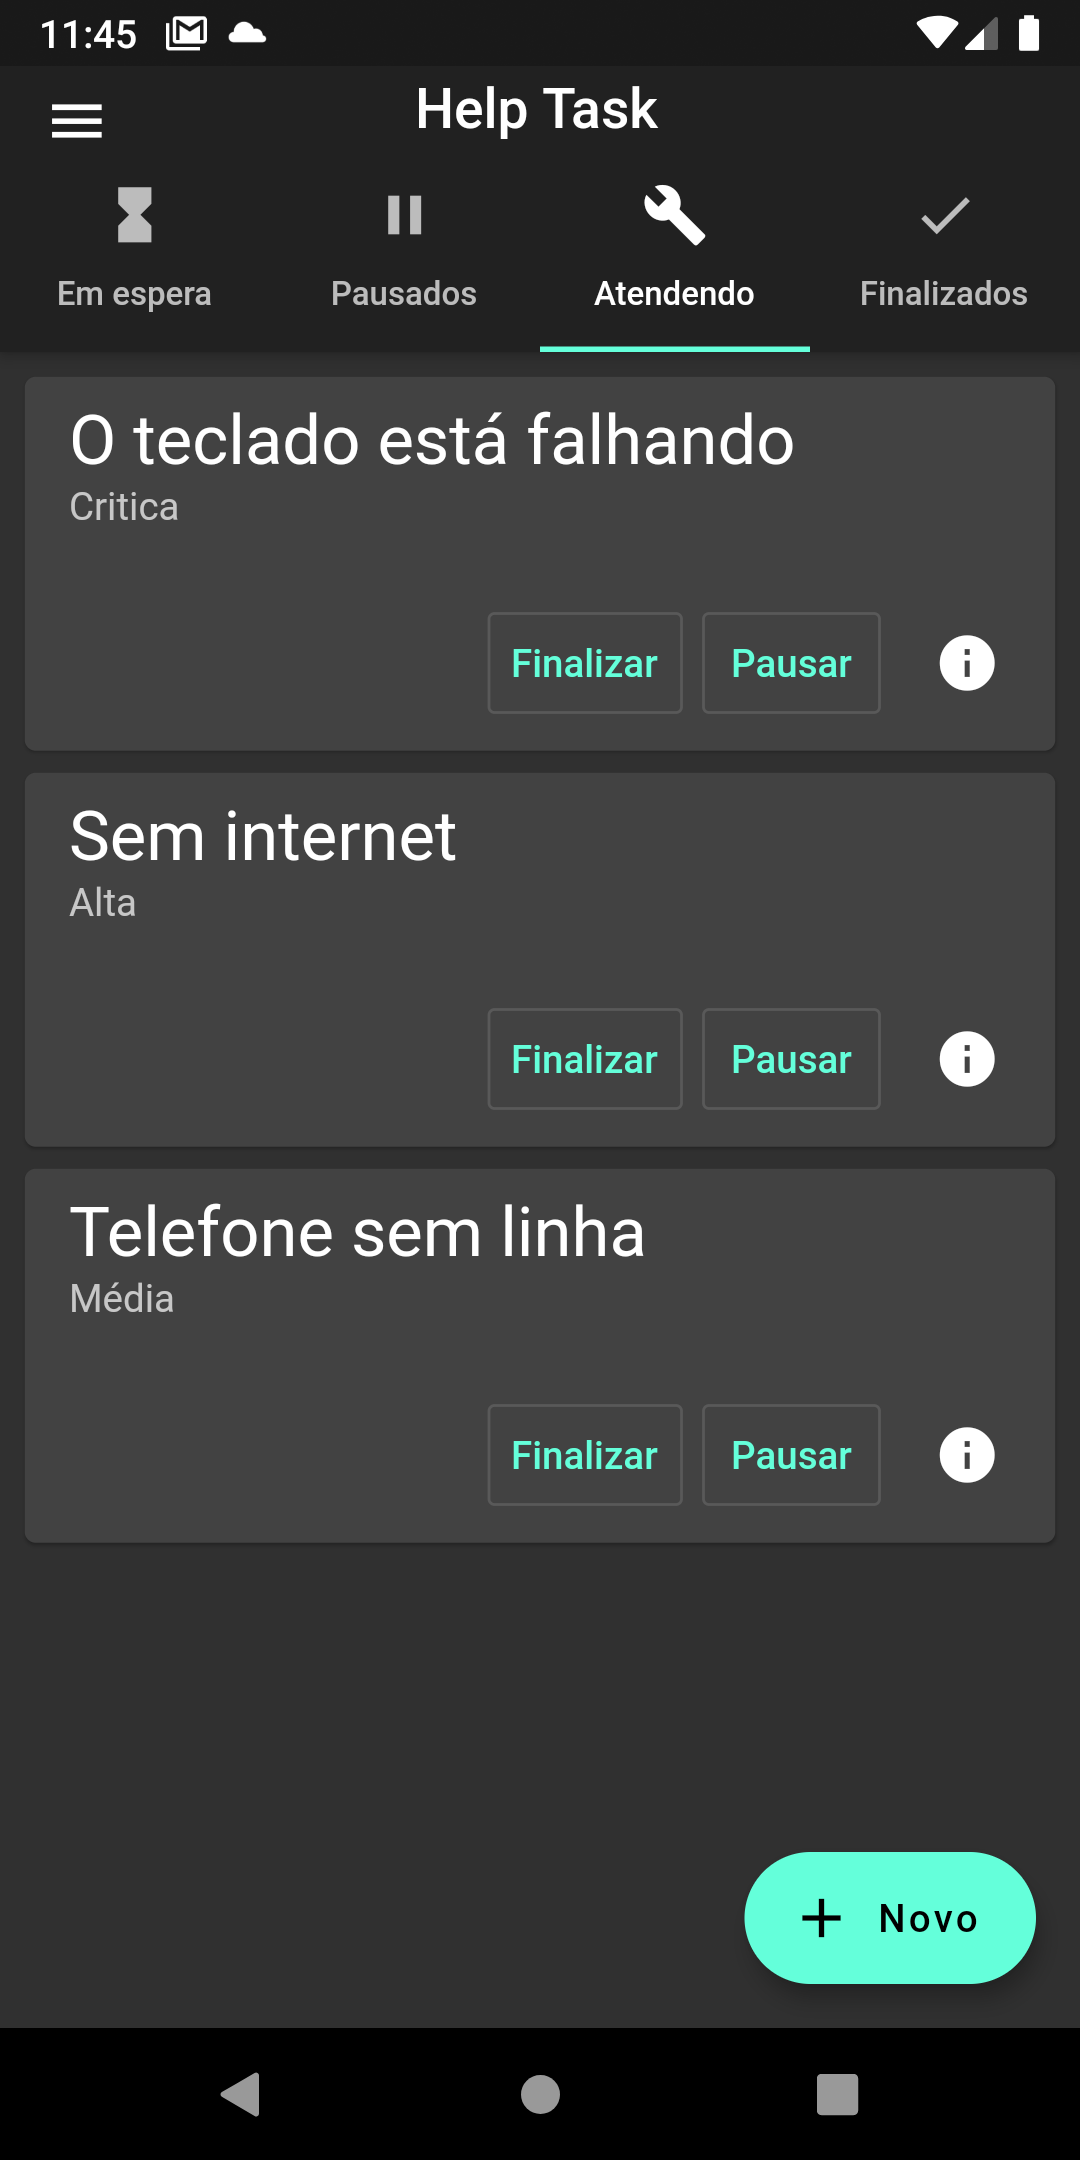
\includegraphics [scale = 0.2]{img/screenshots/4_atendendo.png}}
     \end{frame}
     \label{fig:4_atendendo}
 \end{figure}
\newpage

Na aba de chamados finalizados, conforme a Figura \ref{fig:5_finalizado}, se localizam os chamados que já foram atendidos e finalizados.
\begin{figure}[htb]
     \caption{Print de tela 5 - Lista de chamados finalizados}
     \centering
     \begin{frame}{
     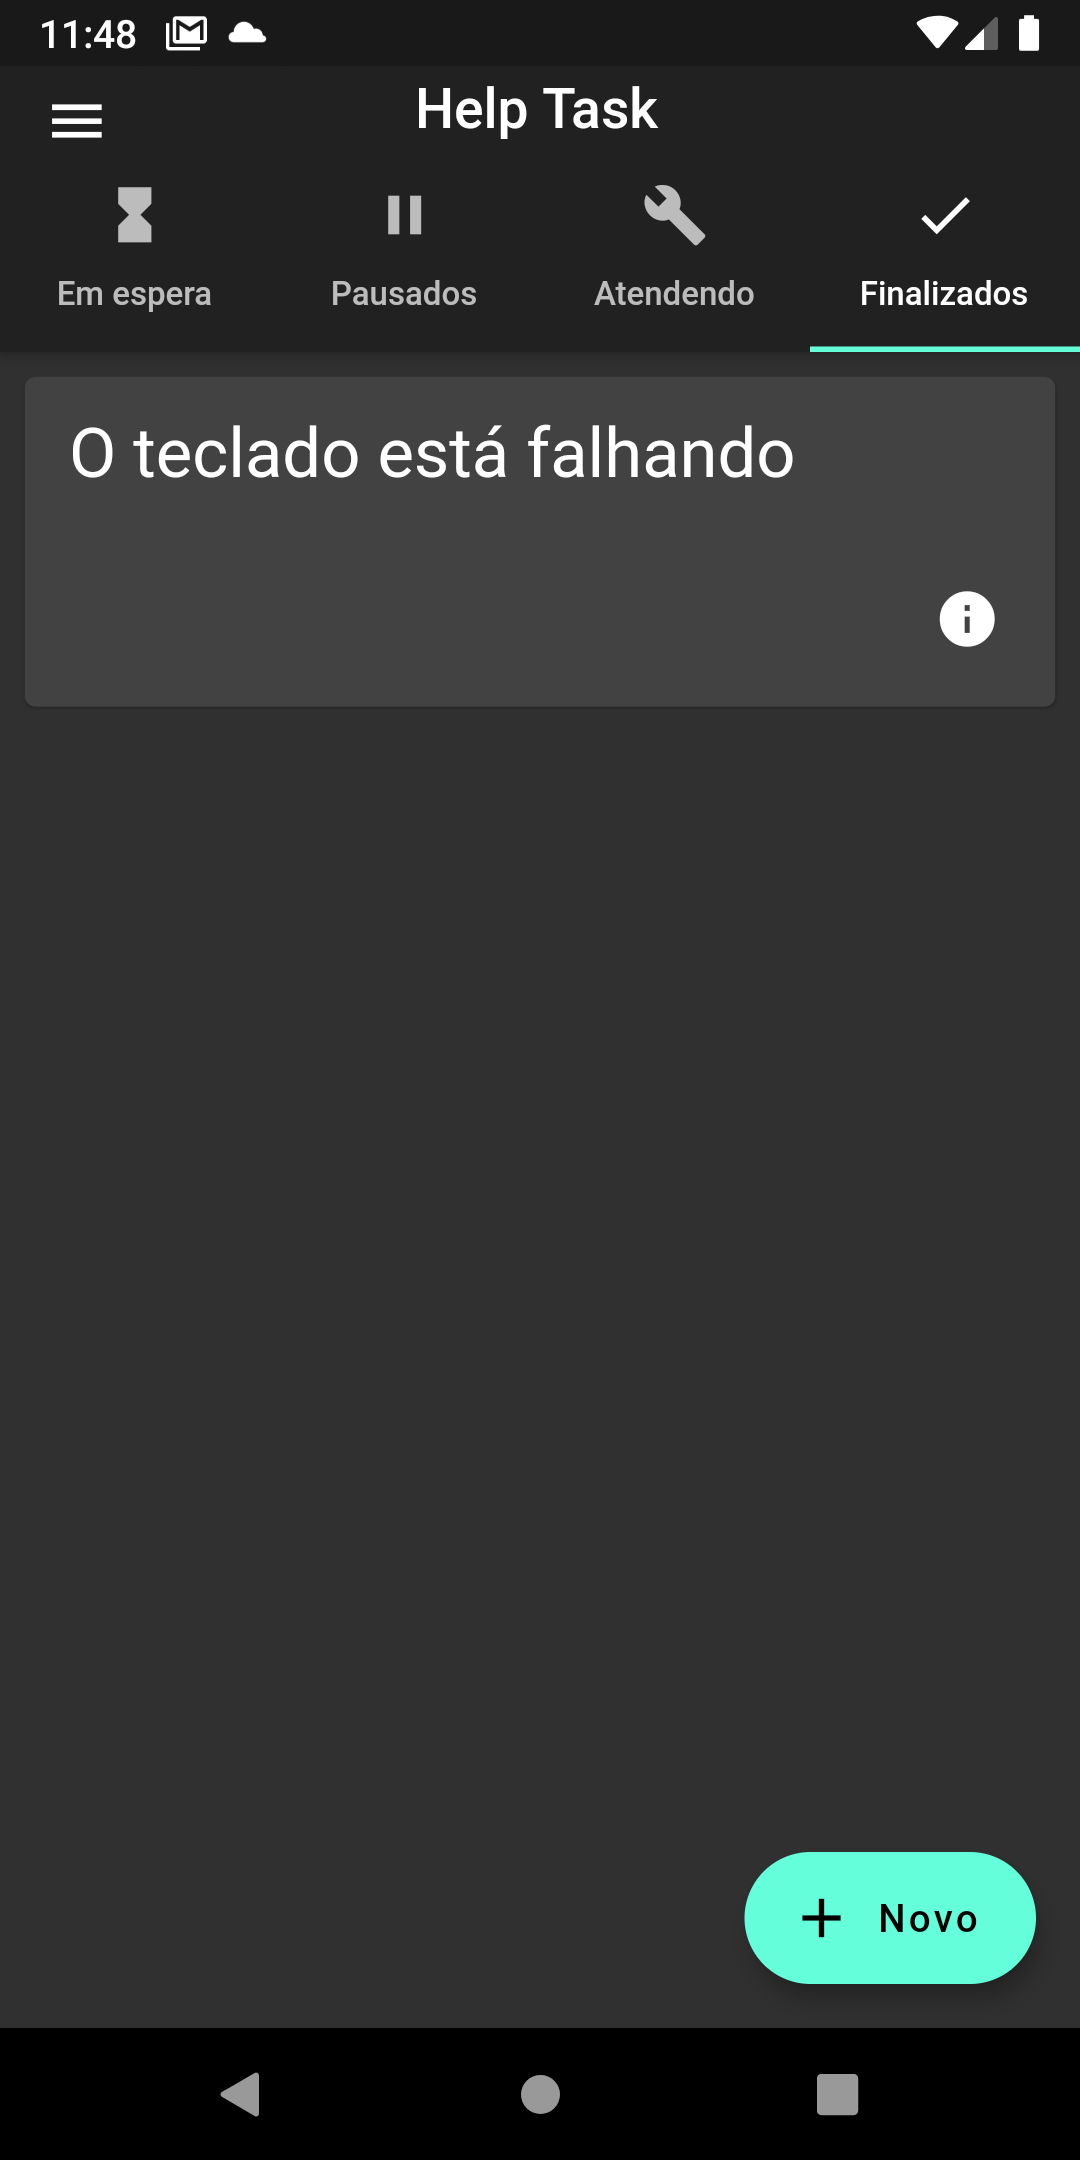
\includegraphics [scale = 0.2]{img/screenshots/5_finalizado.png}}
     \end{frame}
     \label{fig:5_finalizado}
 \end{figure}
\newpage

Em cada \textit{card} de chamado há um ícone de informações, localizado na parte inferior direita do mesmo. Esse ícone se clicado exibe as informações referentes a esse chamado, se os detalhes forem visualizados na tela de finalizados, serão exibidas todas as informações como classificação, tipo, descrição, momento de abertura e resolução. conforme a figura \ref{fig:detalhes}

\begin{figure}[htb]
     \caption{Print de tela 6 - Informações do chamado}
     \centering
     \begin{frame}{
     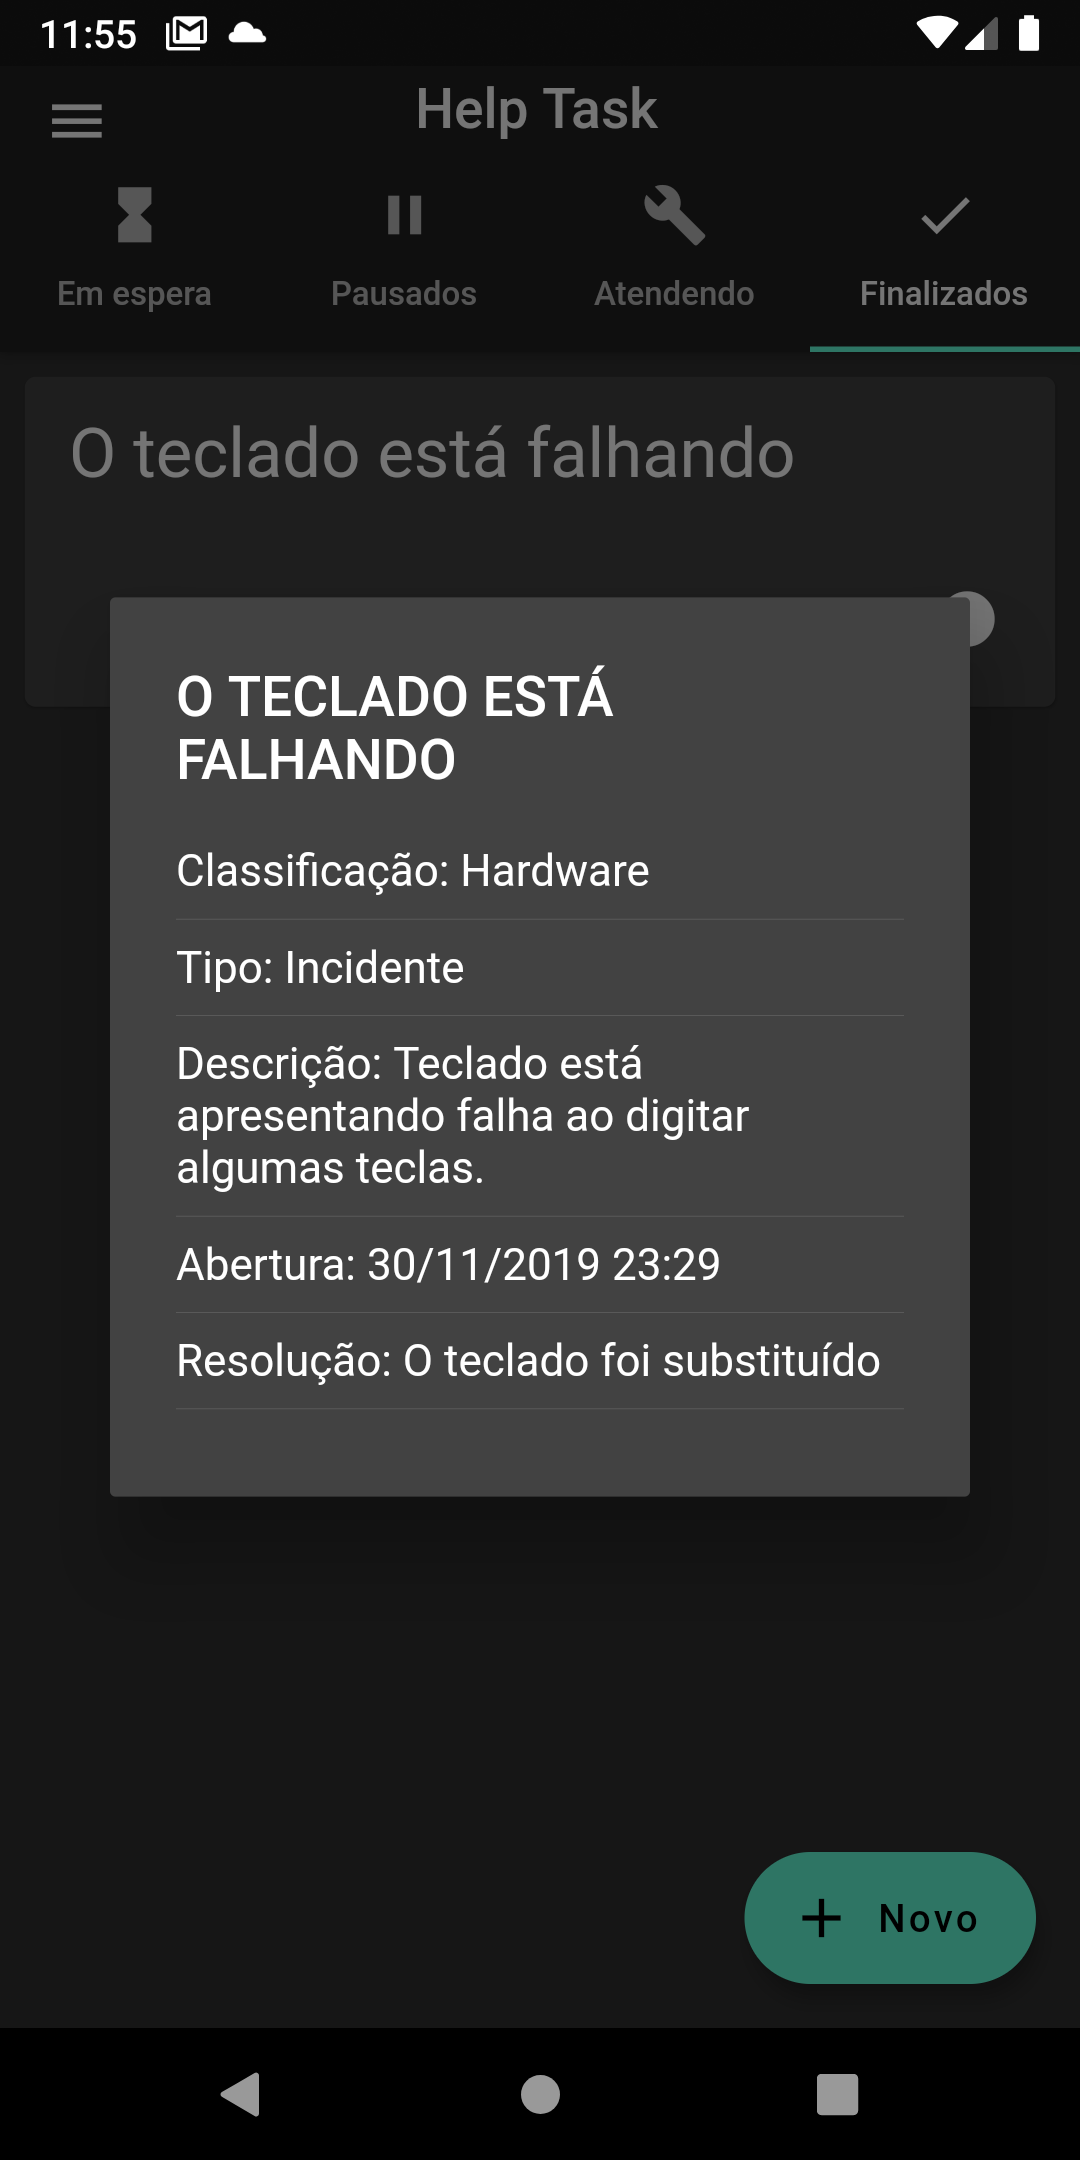
\includegraphics [scale = 0.2]{img/screenshots/detalhes.png}}
     \end{frame}
     \label{fig:detalhes}
 \end{figure}
\newpage


No menu lateral do app, localizam-se as informações do usuário logado como foto de perfil e e-mail. Também encontram-se os botões que levam até a tela de ajuda, onde se encontra uma visualização da documentação do app para o usuário, igual a presente no Apêndice C deste relatório. Também é possível acessar a tela de estatísticas, criar um novo usuário administrador ou fazer logout da sessão.
\begin{figure}[htb]
     \caption{Print de tela 7 - Menu lateral}
     \centering
     \begin{frame}{
     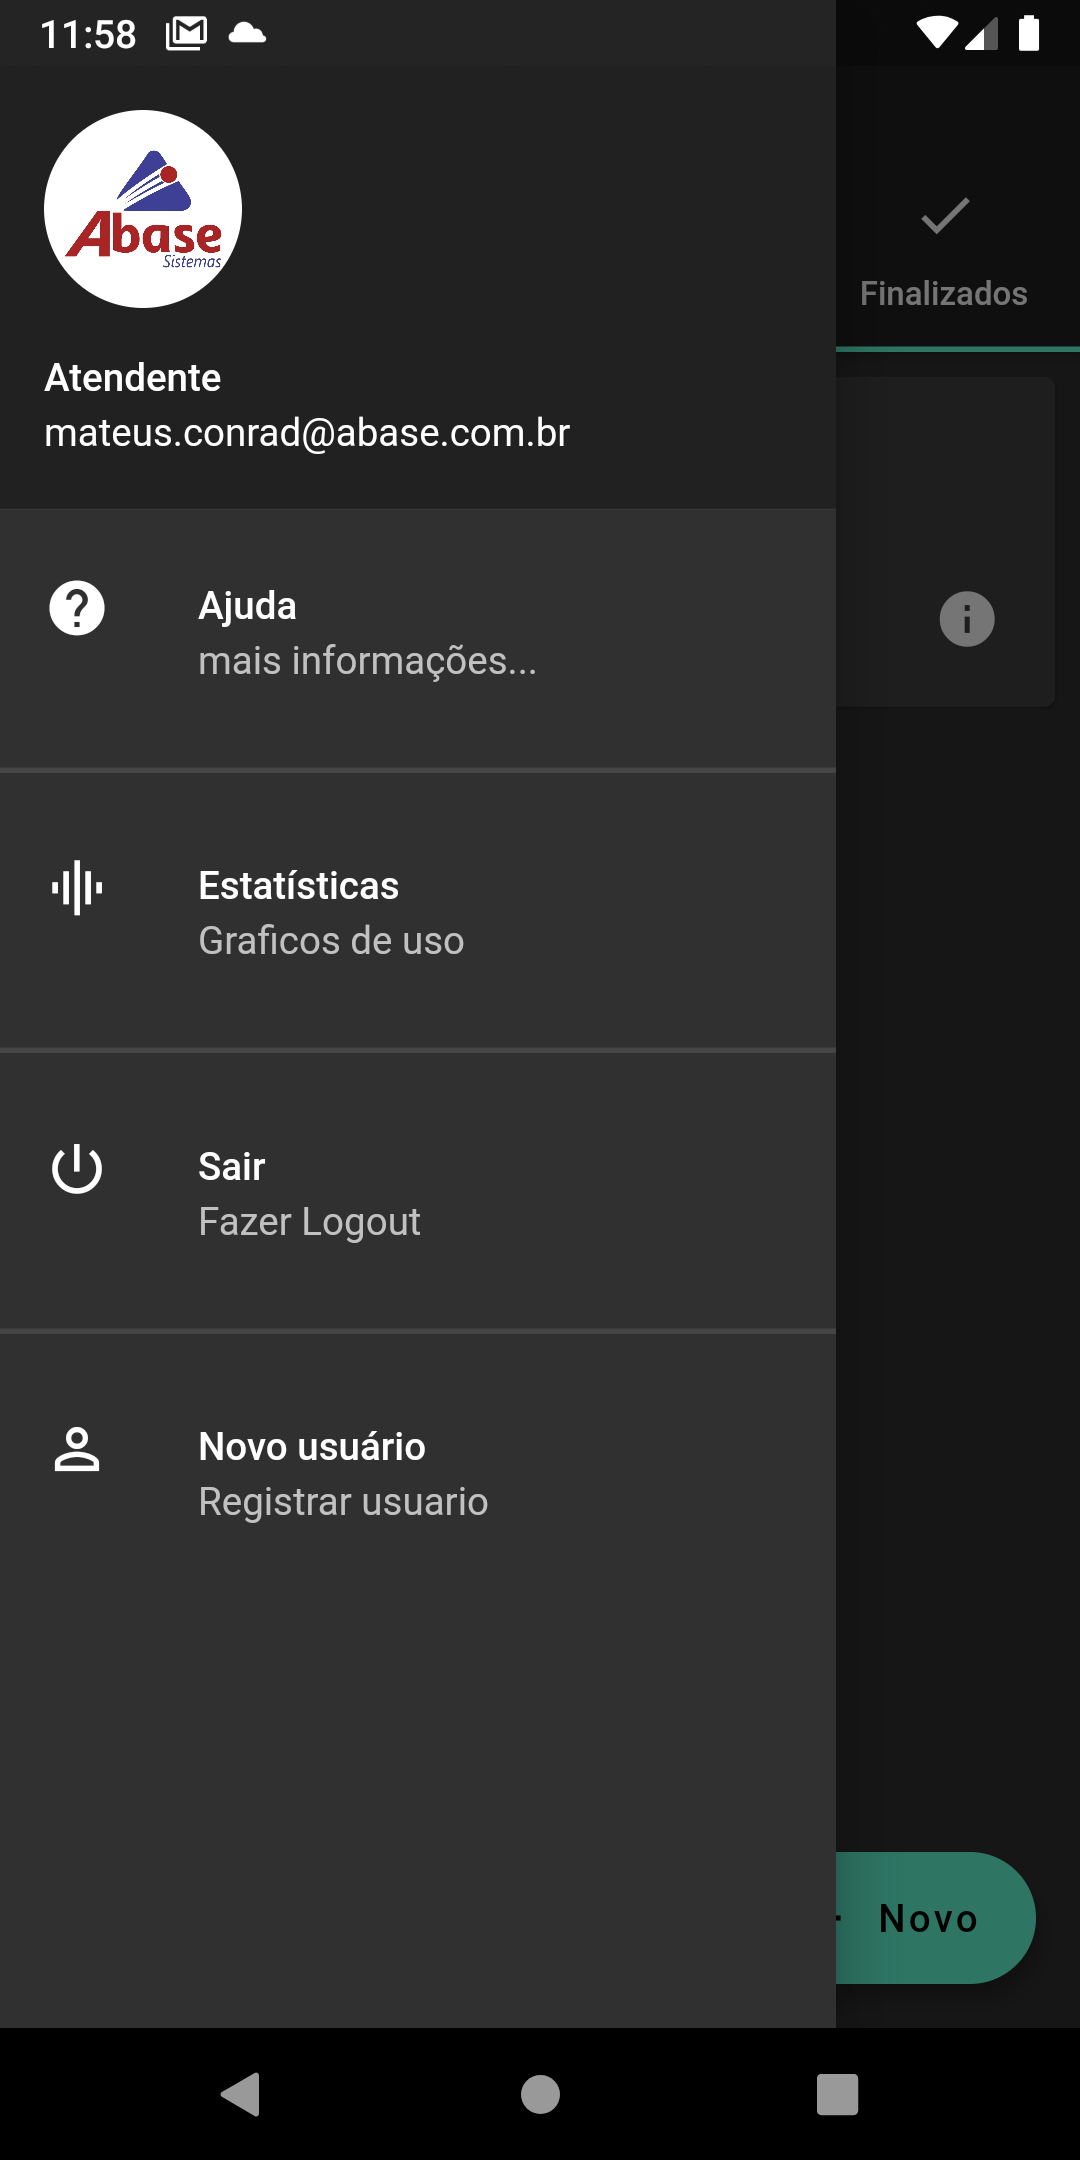
\includegraphics [scale = 0.2]{img/screenshots/6_drawer.png}}
     \end{frame}
     \label{fig:6_drawer}
 \end{figure}
 \newpage
 
 Na tela de abertura de chamado, acessada pelo \textit{Floating Action Button} presente na tela principal, permite colocar um título, descrição, prioridade, classificação e uma foto, conforme a descrição do RF1.
 \begin{figure}[htb]
     \caption{Print de tela 8 - Tela de abrir chammado}
     \centering
     \begin{frame}{
     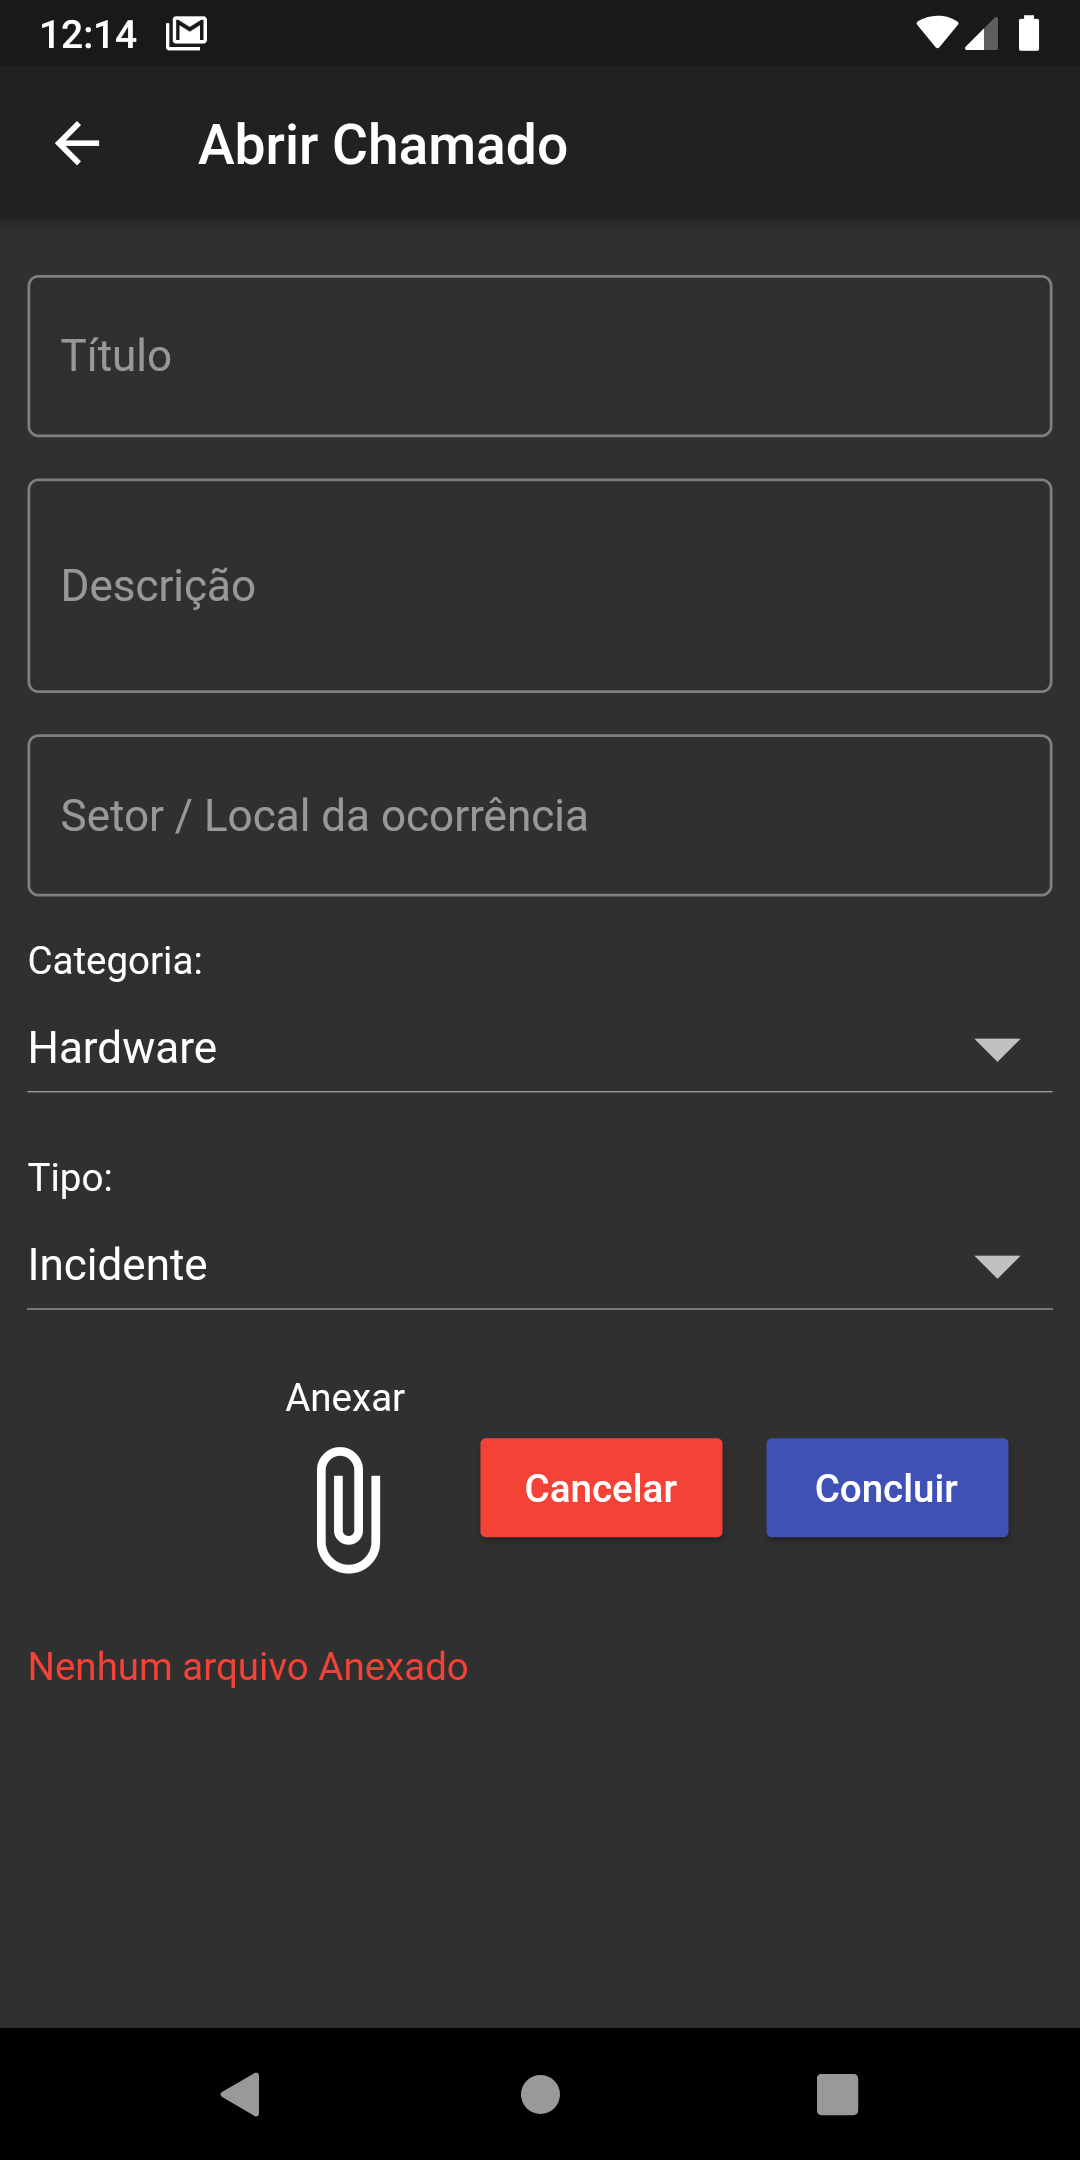
\includegraphics [scale = 0.2]{img/screenshots/7_abrir_chamado.png}}
     \end{frame}
     \label{fig:7_abrir_chamado}
 \end{figure}
 
 Na aba de chamados em espera, é possível atender o chamado ou finalizar o mesmo diretamente. Para atender o chamado é necessário informar uma prioridade, da mesma forma que ao finalizar o chamado é necessário descrever a resolução do mesmo.
\newpage

\section{Arquitetura de Desenvolvimento}
Devido a baixa complexidade tanto na estrutura proposta na análise do aplicativo como no desenvolvimento usando Flutter junto com o Firebase, não se fez necessário o uso de uma padronização de código, como por exemplo a MVC (\textit{Model, View and Controller}) onde o código é separado na parte de \textit{frontend}, operações de \textit{backend} e operações com banco de dados. Parte disso se deve ao não desenvolvimento de uma API, mas sim fazendo uso do Firebase como um \textit{BaaS} e \textit{Storage}.

Como organização do código, foi definido que a maneira mais simples de controlar a organização seria definir cada tela como uma classe dart e também na própria classe, criar métodos para simplificar o entendimento do código.

Como o método \textit{main()} apenas chama a classe \textit{Login()}, essa é a tela que será exibida ao abrir o aplicativo. Exemplificando, ainda usando a classe \textit{Login()} como exemplo, no código desta há a declaração da classe em si, que se dá por um \textit{Stateful Widget} e seu conteúdo dentro de um Widget chamado Scaffold, como pode ser observado no trecho de código 2. O Scaffold contém apenas chamadas para os métodos que exibem a imagem de logo, título do app e campos de login, esse mesmo estilo de programação foi usado em todo o código.
\begin{lstlisting}[numbers=left, language=Java, style=mycode, caption={Trecho de Código página de Login}, label={lst:loginpage-code}]
class Login extends StatefulWidget {
  @override
  _LoginState createState() => _LoginState();
}
class _LoginState extends State<Login> {
/*aqui se inclui todo o resto do codigo da classe, como declaracao de variaveis, metodos e os Widgets*/ 
}
\end{lstlisting}
\source{Adaptado do repositório do github.com/mateusconrad/app\_suporte}
\justifying\setlength{\parindent}{1,25cm} 

\newpage
Na figura \ref{fig:arquitetura_lib}, pode-se observar a estrutura de arquivos que compõem a pasta lib. Essa é a pasta padrão de um projeto flutter para os arquivos das classes. A pasta lib foi divida em outras três pastas e também contém 3 arquivos em sua raíz, sendo respectivamente as pastas "\textit{drawer}", "\textit{tabs}", "telas" e os arquivos \textit{home}, \textit{login} e \textit{main}.

 \begin{figure}[htb]
     \caption{Classes diretório Lib}
     \centering
     \begin{frame}{
     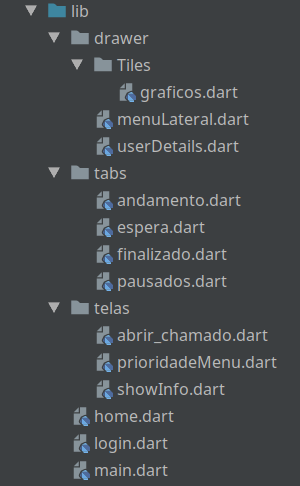
\includegraphics [scale = 0.8]{img/arquitetura_lib}}
     \end{frame}
     \label{fig:arquitetura_lib}
 \end{figure}

Começando pelos arquivos na raíz da pasta lib, há o arquivo main, que contém o método principal para inciar o aplicativo. O código contido no arquivo main faz uma chamada para abrir a tela de login, que dessa forma se identifica como a página principal do aplicativo, conforme o trecho de código 3.

\newpage

\begin{lstlisting}[numbers=left, language=Java, style=mycode, caption={Trecho de Código página do main()}, label={lst:main-code}]
void main() {
  runApp(MaterialApp(
    debugShowCheckedModeBanner: false,
    home: Login(), //chamada para pagina de login
  ));
}

\end{lstlisting}
\source{Adaptado do repositório do github.com/mateusconrad/app\_suporte}
\justifying\setlength{\parindent}{1,25cm} 

Quando o usuário é autenticado pela página de login, o mesmo é redirecionado para a página Home, identificada pelo arquivo \textit{home.dart} e por sua classe \textit{TabBarHome()}. O método de login com redirecionamento pode ser conferido no trecho de código 4.

\begin{lstlisting}[numbers=left, language=Java, style=mycode, caption={Trecho de Código do método de login}, label={lst:signin-code}]

final GoogleSignInAccount googleUser = await _googleSignIn.signIn();
final GoogleSignInAuthentication googleAuth = await googleUser.authentication;
final AuthCredential credential = GoogleAuthProvider.getCredential(
  accessToken: googleAuth.accessToken,
  idToken: googleAuth.idToken,);
FirebaseUser userDetails = (await _auth.signInWithCredential(credential));
ProviderDetails providerInfo = new ProviderDetails(userDetails.providerId);
List<ProviderDetails> providerData = new List<ProviderDetails>();
providerData.add(providerInfo);
UserDetails details = new UserDetails(userDetails.providerId, userDetails.displayName, userDetails.photoUrl,userDetails.email,providerData,);
final user = UserDetails;
Navigator.pushReplacement(context,
    new MaterialPageRoute(builder: (context) => new TabBarHome(),),);
    return userDetails;
  }
\end{lstlisting}
\source{Adaptado do repositório do github.com/mateusconrad/app\_suporte}
\justifying\setlength{\parindent}{1,25cm} 

\newpage
\section{Estrutura dos dados e autenticação}
No que diz respeito a estrutura de dados, foi usado a forma que o próprio Firebase disponibiliza, a de banco orientada a documentos, onde há níveis de hierarquia entre coleções, documentos e campos. A figura \ref{fig:firestore1} exibe como fica a estrutura dos dados gerados da abertura ate a finalização de um chamado, onde há a coleção de chamados, listando todos os ID's de todos os chamados cadastrados e também exibindo todos os campos do chamado selecionado.

    \begin{figure}[htb]
        \caption{Dados de um chamado}
        \centering
        \begin{frame}{
        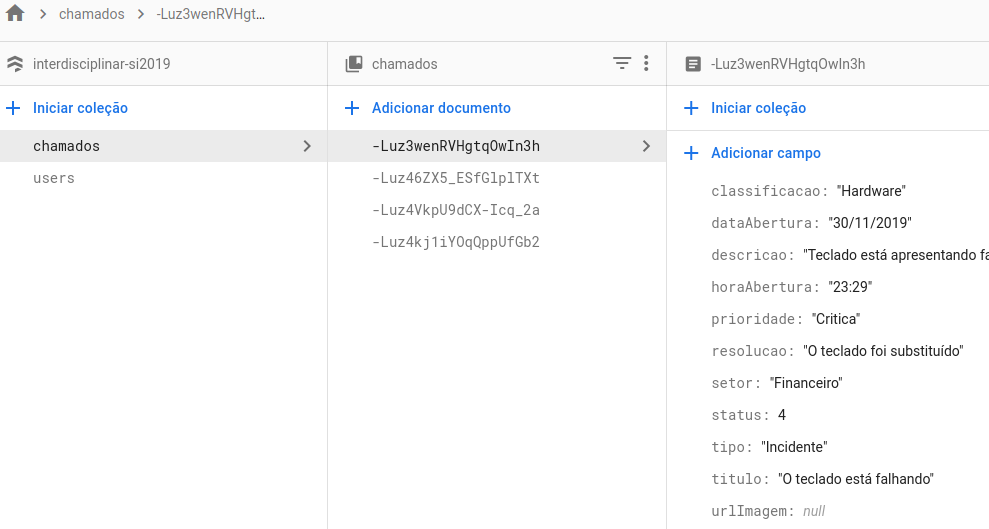
\includegraphics [scale = 0.44]{img/firestore1.png}}
        \end{frame}
        \label{fig:firestore1}
    \end{figure}

Assim como os chamados, os dados dos atendentes ficam registrados em banco. Os dados dos usuários são capturados através do método de \textit{Authentication} do firebase, onde foram habilitados os provedores de email e também o do google.   
    
    \begin{figure}[htb]
        \caption{Firebase Authentication}
        \centering
        \begin{frame}{
        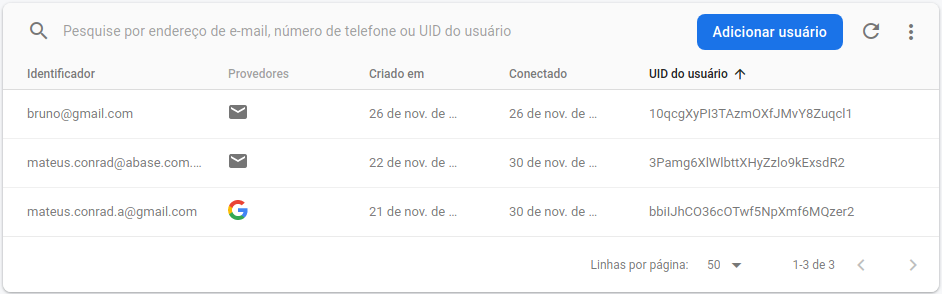
\includegraphics [scale = 0.455]{img/firestore2.png}}
        \end{frame}
        \label{fig:firestore2}
    \end{figure}


\section{Testes e Qualidade de Software}
Não foi aplicado nenhum tipo de teste de software como testes de unidade ou testes com usuários como o BDD( Behaviour Driven Development). Esses testes não foram aplicados devido a falta de tempo hábil para implantação e realização dos mesmos. No entanto ao pesquisar como testes de software podem ser realziados em apps desenvolvidos usando o flutter, chegou-se a informação que o framework em si possui suporte para três tipos de teste, sendo esses: Testes de unidade, teste de \textit{widgets} e teste de integração.
 
De acordo com a documentação do Flutter, os testes de unidade se propõem a testar partes isoladas do código, como funções métodos ou uma classe. Enquanto isso, os testes de Widget tem por função testar um único widget, em outros frameworks esse teste pode ser encontrado pelo nome de teste de componente. Por último, apresenta-se o teste de integração, que possui a tarefa de testar o aplicativo como um todo, ou em casos de aplicações muito grandes, isolar uma parte significativa do aplicativo e testá-la por completo.

A forma que o grupo encontrou de manter um controle sobre erros achados durante o desenvolvimento foi fazer o cadastro de \textit{issues} no repositório do código no github, assim cria-se uma linha de orientação ao momento de desenvolver. As issues funcionam como um cadastro de erros, problemas e melhorias a serem feitas no código. Todas as issues cadastradas que foram abertas ou fechadas podem ser verificadas em: <https://github.com/mateusconrad/app\_suporte/issues>, conforme a figura \ref{fig:issues_github}.
    
 \begin{figure}[htb]
     \caption{Issues Github}
     \centering
     \begin{frame}{
     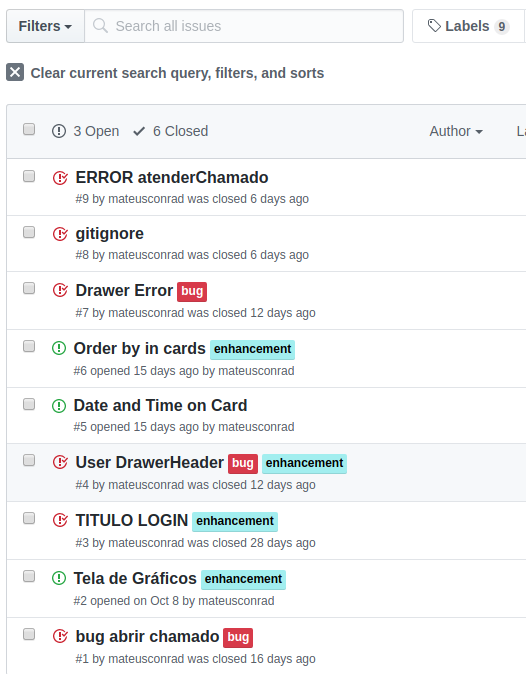
\includegraphics [scale = 0.6]{img/issues_github}}
     \end{frame}
     \label{fig:issues_github}
 \end{figure}
    
\chapter*{Conclusão} \label{chap:concl}


Partindo, então do tema do trabalho, o qual tratava do desenvolvimento de um app mobile para chamados de suporte de uma empresa, podem se apresentar as conclusões sobre a análise realizada e o aplicativo desenvolvido.

Primeiramente, retomando os  objetivos estipulados neste trabalho, os quais traziam como objetivo geral desenvolver um aplicativo para padronizar o processo de abertura de chamados de suporte internos de uma empresa de TI pode-se verificar que este foi parcialmente cumprido, pois a aplicação foi desenvolvida e funciona, por outro lado não sofreu um período de testes de uso ou aceitação dos próprios usuários e atendentes.

Em sequência, como objetivos específicos foram propostos a realização da análise e desenvolvimento de um app para chamados de suporte, utilização de banco de dados em tempo real para gerenciamento dos dados, realizar os testes de software no aplicativo e disponibilizar o arquivo para instalação do app. Foram atingidos e concluídos os três primeiros, não houve a realização dos testes de software devido a limitações de desenvolvimento do grupo, bem como a falta de tempo para a realização e documentação dos mesmos. 

O app também não foi disponibilizado ou hospedado em lojas de aplicativos pois há custos para isso que não foram previstos e também não se viu a necessidade, pois o código do aplicativo já é aberto.

A partir do problema levantado na fase de análise, o qual questionava como um aplicativo pode padronizar e agilizar o processo de abertura de chamados de suporte internos de uma empresa, foram levantadas duas hipóteses para responder ao problema.

A primeira hipótese afirmava que O aplicativo desenvolvido pode definir uma padronização para os chamados de suporte interno na empresa. A primeira hipótese, pôde ser corroborada apesar da implantação da aplicação não ter ocorrido, pois pode se observar que a metodologia empregada é capaz de padronizar a maneira de realizar e requisitar os chamados de suporte internamente na empresa, conforme a apresentação do software presente na seção 4 do capítulo 3. O último passo efetivo para este ponto é a própria empresa tratar o app como o único canal de comunicação entre usuário e suporte. Os testes foram somente realizados pelos pesquisadores na medida em que a construção do app evoluiu. Quanto ao quarto objetivo, não pode ser atingido, pois o app foi disponibilizado somente na forma de código-fonte, ao contraponto da proposta de fornecer o arquivo de instalação.

Já a segunda hipótese afirmava que o aplicativo desenvolvido permite visualizar estatísticas de chamados realizados". Essa hipótese não pode ser corroborada nem refutada, uma vez que não houve a implementação necessária, ou seja, não houve a aplicação de gráficos em relação as informações dos próprios chamados, não houve tempo hábil para a implementação dos mesmos, como também não houve a definição de um escopo de quais informações esses gráficos iriam exibir em tela.

A análise foi realizada tendo como base a Abase Sistemas, como ponto mais específico, em seu setor responsável pela infraestrutura do ambiente, formulando assim uma aplicação que fosse capaz de gerir os chamados de suporte.

A partir dos pontos de melhoria ou que ficaram fracos no desenvolvimento do aplicativo, podem ser elencadas algumas propostas futuras, sendo essas: a disponibilização do aplicativo nas lojas \textit{App Store} e \textit{Play Store}, implementar a geração de gráficos e filtros baseados em ordenamento de data, título, prioridade e tipo de chamado, a realização da implementação dos gráficos dos chamados, e também a implementação de de um chat dentro da aplicação, assim permitindo, além da abertura do chamado, uma breve comunicação entre atendente e usuário para evitar erros.

Por meio do desenvolvimento da aplicação proposta, a qual propunha a padronização dos chamados de TI através de um app mobile para sistemas operacionais Android, pode ser observada a necessidade de um fluxo de processos bem estruturado para que a eficiência da equipe de TI cumprisse adequadamente seu papel.

O desenvolvimento da presente pesquisa foi capaz agregar novos conhecimentos aos pesquisadores, tanto no que diz respeito aos conteúdos da disciplina de Linguagem de Programação III e Análise e Estratégias Sistemas, quanto na construção de conhecimentos acerca da área de suporte das empresas, portanto, considera-se que foi de grande valia o aprendizado em relação a duas áreas da tecnologia que apesar de serem diferentes uma da outra, puderam agregar valor aos acadêmicos unindo conceitos de desenvolvimento mobile com gerenciamento de TI.

\bibliographystyle{template/abnt-pt}
\bibliography{bib/bibliography}
\clearpage

\appendix
\renewcommand{\thechapter}{APÊNDICE I -}
\chapter{Orçamento}
O quadro \ref{tab:my_table_orcamento} prevê os custos que o trabalho terá. Os custos envolvem as cópias para impressão, mensalidade do curso partir dos créditos matriculados e o total como soma de ambos.
\begin{table}[htb]
    \caption{Orçamento}
    \label{tab:my_table_orcamento}
    \centering
    \begin{tabular}{|c|c|}
        \hline
         Despesa & Valor \\ 
         \hline
         Cópias & R\$ 50,00\\
         \hline
         Mensalidade & R\$ 6813,12\\
         \hline
         Desenvolvimento & R\$ 10000,00\\
         \hline
         TOTAL & R\$ 16863,12\\
         \hline
    \end{tabular}
\end{table}

\renewcommand{\thechapter}{APÊNDICE II -}
\chapter{Cronograma de Atividades} \label{sec:schedule_activities_table}
 
O Quadro \ref{tab:my_table_cronograma} ilustra o cronograma de atividades. As células marcadas com "X"\ representam as atividades realizadas e as células marcadas com o fundo cinza representam as atividades realizadas. As células marcadas com "X"\ e fundo cinza representam as atividades que foram propostas e realizadas.

\begin{table}[htb]
    \caption{Cronograma das atividades}
    \label{tab:my_table_cronograma}
    \centering
    % \resizebox{\textwidth}{!}{%
    \begin{tabular}{|c|c|c|c|c|c|c|}
        \hline 
         Tarefa / Mês & JUL & AGO & SET & OUT & NOV & DEZ\\ 
         \hline
         Elaboração do projeto & X\cellcolor{gray!50}  & & & & &\\
         \hline
         Elaboração do Referencial & & X\cellcolor{gray!50} & X\cellcolor{gray!50} & & &\\
         \hline
         Entrega do Projeto & &  & X\cellcolor{gray!50} & & &\\
         \hline
         
         Desenvolvimento do App & & & X \cellcolor{gray!50}& X\cellcolor{gray!50} & X\cellcolor{gray!50} &  \\
         \hline
         Documentar Resultados & & & & & X\cellcolor{gray!50} & X\cellcolor{gray!50}\\
         \hline
         Apresentação Resultados & & & & & X\cellcolor{gray!50} & X\cellcolor{gray!50}\\ 
         \hline
    \end{tabular}
    % }
\end{table}

\renewcommand{\thechapter}{APÊNDICE III -}
\chapter{Documentação de usuário}

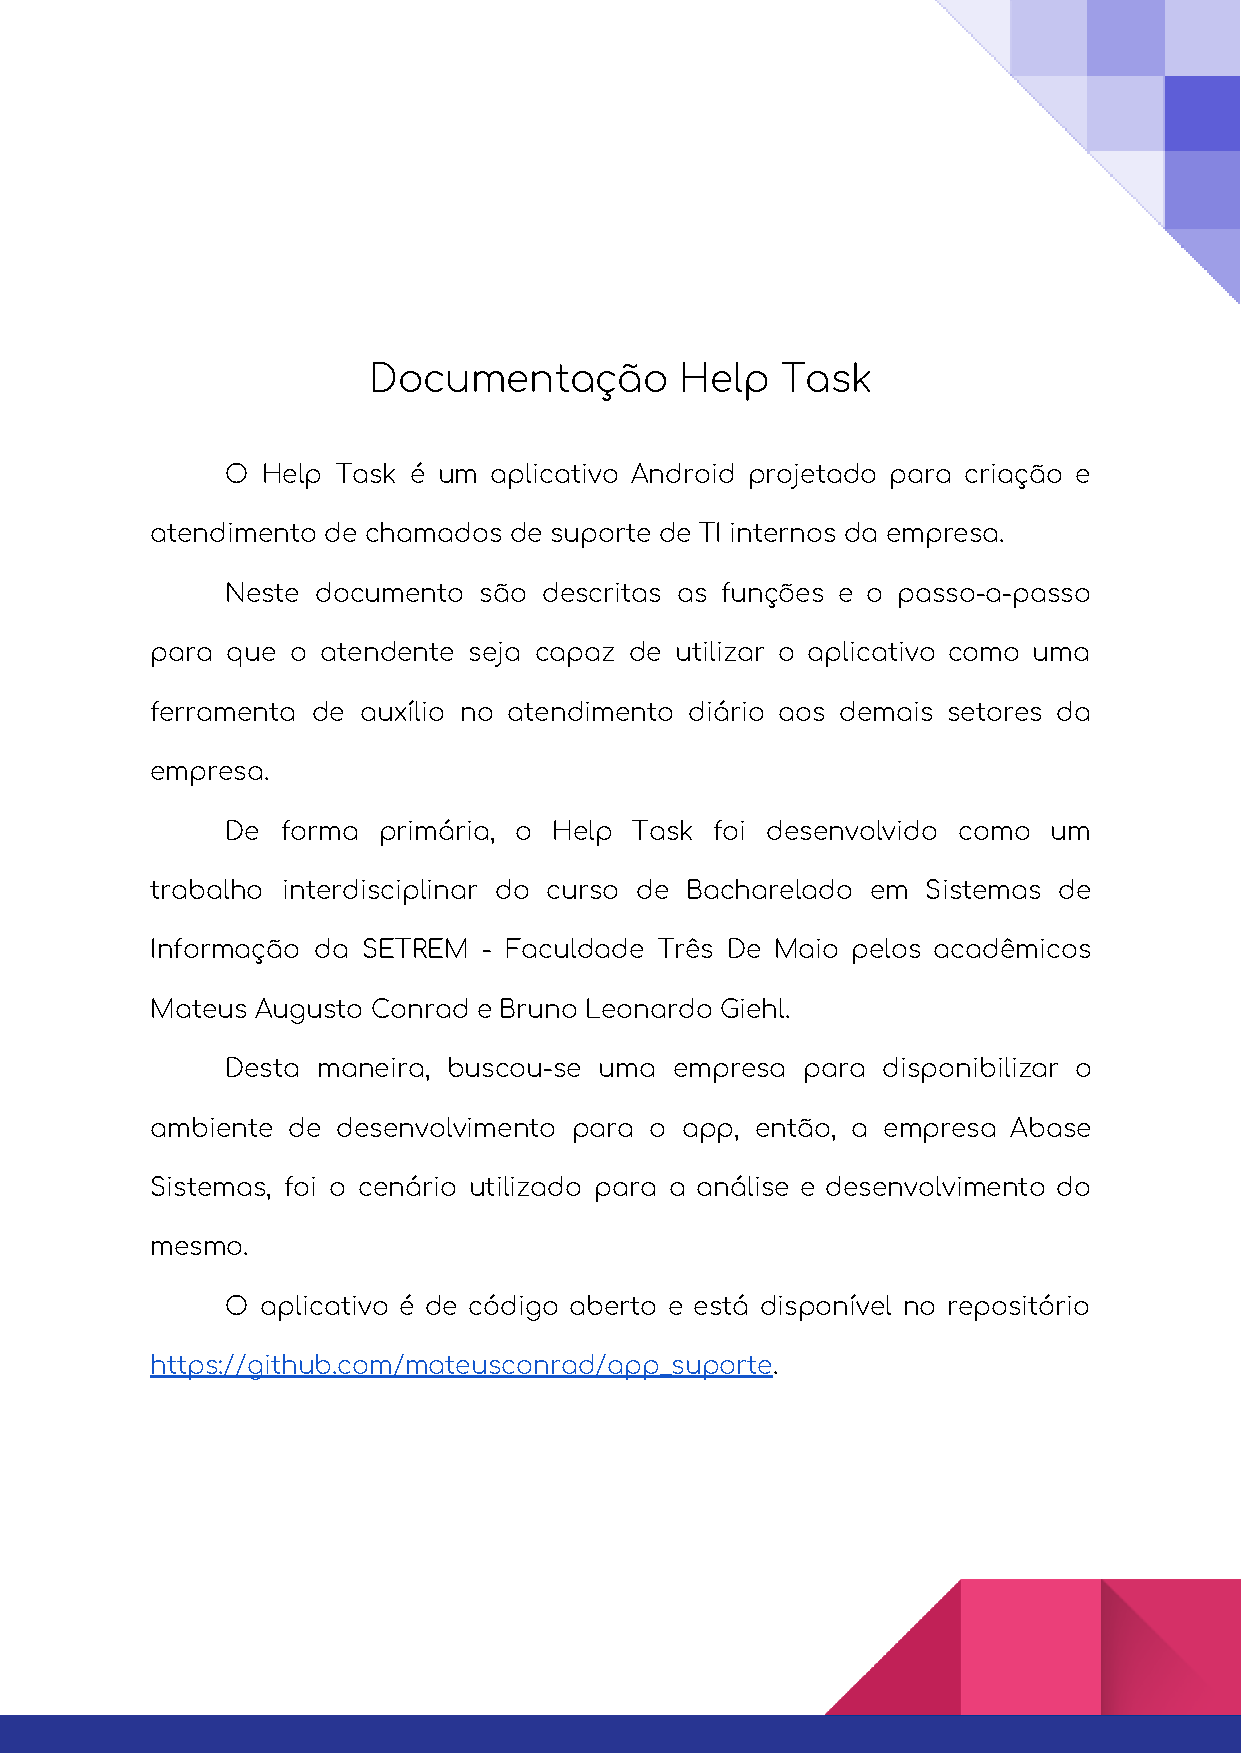
\includepdf[page={-}]{documentacao}

\renewcommand{\thechapter}{APÊNDICE IV -}
\chapter{Resumo Expandido}

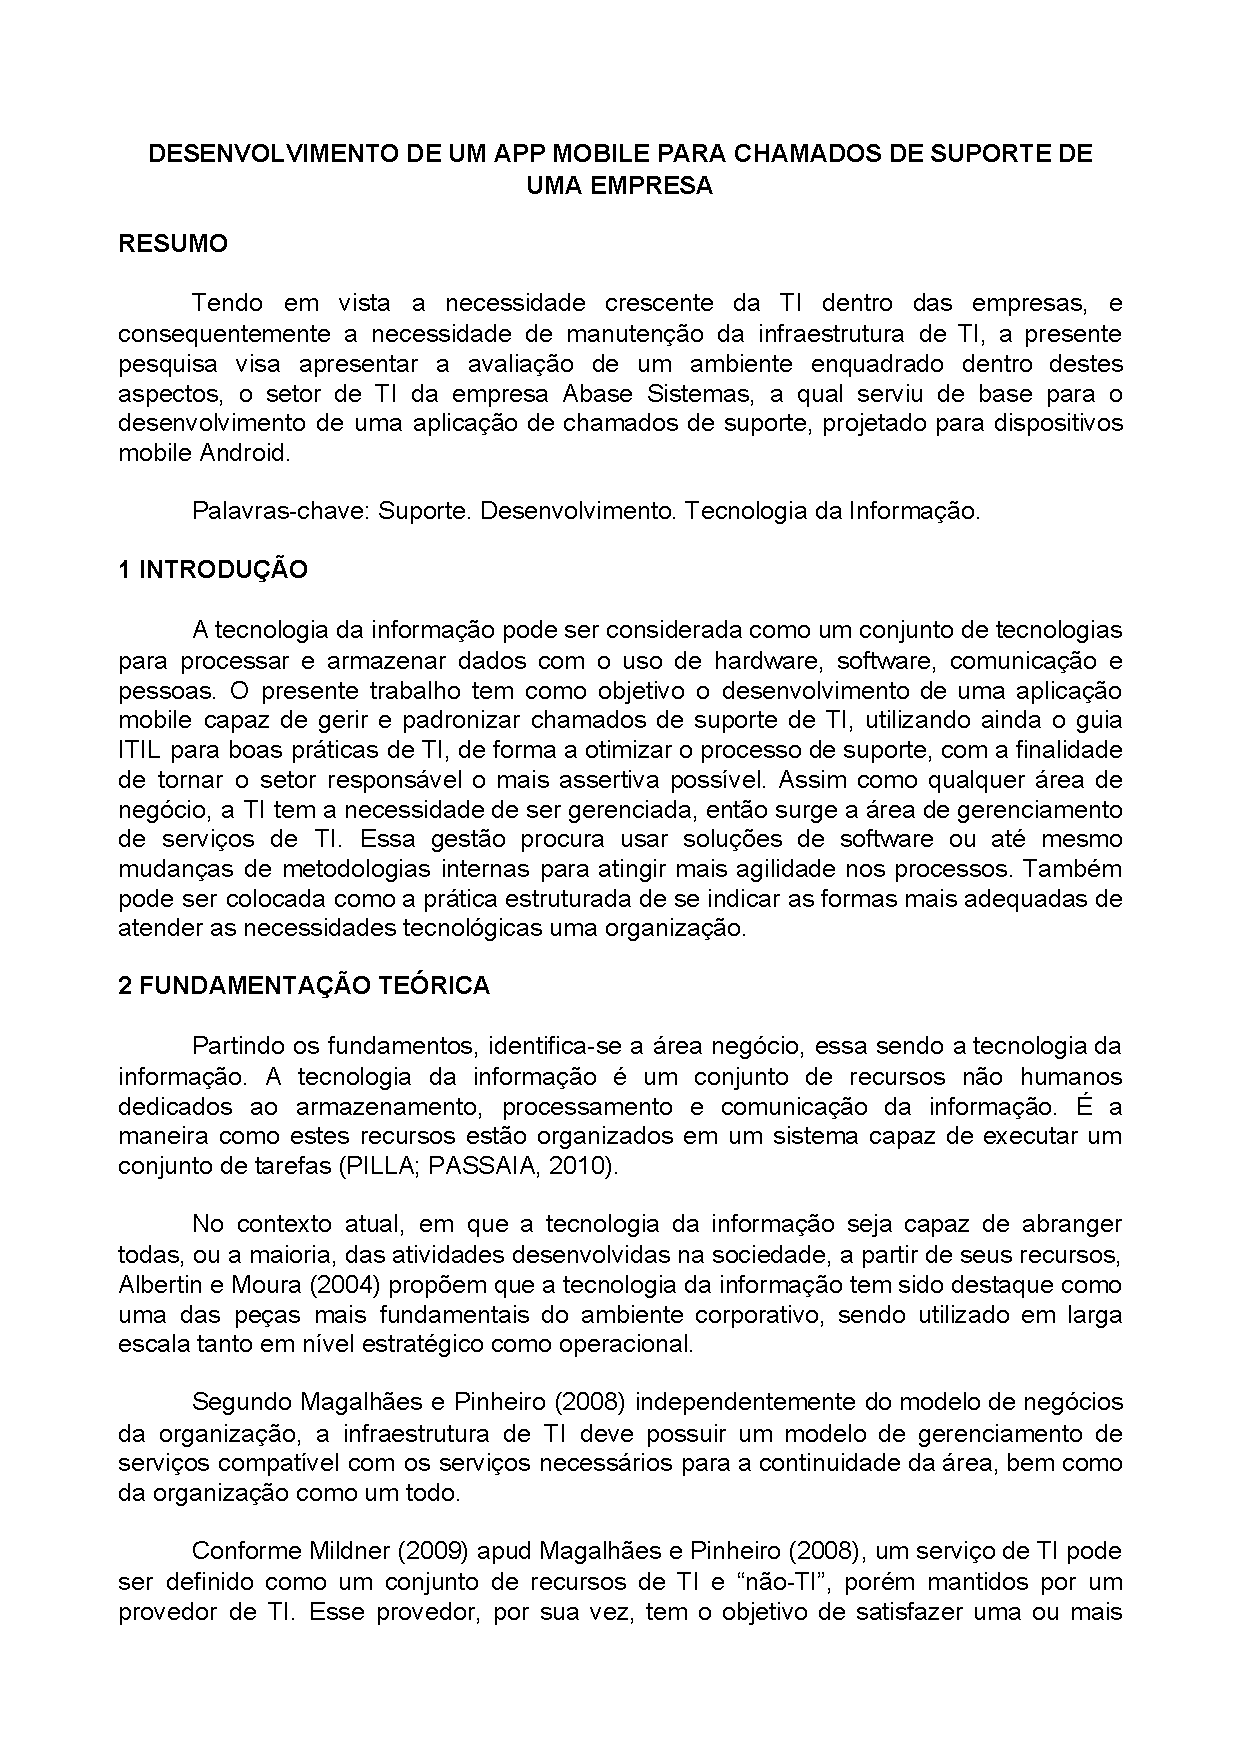
\includepdf[page={-}]{expandido}


\end{document}

